\documentclass[conference]{IEEEtran}
\IEEEoverridecommandlockouts
\usepackage{cite}
\usepackage{amsmath,amssymb,amsfonts}
\usepackage{algorithmic}
\usepackage{graphicx}
\usepackage{textcomp}

\usepackage{subfig}
\usepackage{url}
% \usepackage{hyperref}
% I don't want the borders of hyper links
\usepackage[hidelinks]{hyperref} 
\usepackage{xcolor}
\usepackage{txfonts}
\usepackage{pifont}

%\usepackage{bbding}
\usepackage{multirow}
\usepackage{makecell}
\usepackage[justification=centering]{caption}
\usepackage{xspace}
\usepackage{comment}
\usepackage{listings}
\usepackage{tikz}
\usepackage{calc}
%\usepackage{fancyvrb}
\usepackage[keeplastbox]{flushend}

\def\BibTeX{{\rm B\kern-.05em{\sc i\kern-.025em b}\kern-.08em
    T\kern-.1667em\lower.7ex\hbox{E}\kern-.125emX}}

% Ensure letter paper
\pdfpagewidth=8.5in
\pdfpageheight=11in

% \newcommand{\hpcasubmissionnumber}{N69}

\newcommand{\cmark}{\ding{51}}%
\newcommand{\xmark}{\ding{55}}%

\newcommand{\todo}[1]{{\color{red}\bfseries [[#1]]}}
\newcommand{\toconfirm}[1]{{\color{blue}\bfseries #1}}
\newcommand{\TP}[1]{{\color{red}\bfseries [[#1]]}}

\newcommand{\Watcher}{{Watcher}}
\newcommand{\WA}{{Watcher}}
\newcommand{\ASAN}{{ASan}}
\newcommand{\DT}{{DoubleTake}}

\newcommand{\OB}{\texttt{OpenBSD}}
\newcommand{\DieHarder}{\texttt{DieHarder}}
\newcommand{\DL}{\texttt{DLmalloc}}
\newcommand{\JE}{\texttt{jemalloc}}
\newcommand{\NA}{\texttt{NUMAlloc}}
\newcommand{\NM}{\texttt{NUMAlloc}}
\newcommand{\TN}{TCMalloc-NUMA}

\newcommand{\pthread}{\texttt{pthread}}
\newcommand{\pthreads}{\texttt{pthreads}}
\newcommand{\specialcell}[2][c]{%
  \begin{tabular}[#1]{@{}c@{}}#2\end{tabular}}


\pagenumbering{arabic}

\begin{document}

\title{NUMAlloc: A Faster NUMA Memory Allocator} 

% \author{{\normalsize{HPCA 2022 Submission
%       \textbf{\#\hpcasubmissionnumber} -- Confidential Draft -- Do NOT Distribute!!}}}

\maketitle

\begin{abstract}
The NUMA architecture accommodates the hardware trend of an increasing number of CPU cores. It requires the cooperation of memory allocators to achieve good performance for multithreaded applications. Unfortunately, existing allocators \NEW{do not} support NUMA architecture well.
% \todo{Unfortunately, none of the existing allocators can support NUMA architecture well}.
This paper presents a novel memory allocator -- \NM{}, that is designed for the NUMA architecture. \NM{} is centered on a binding-based memory management. On top of it, \NM{} proposes an ``origin-aware memory management'' to ensure the locality of memory allocations and deallocations, as well as a method called ``incremental sharing'' to balance the performance benefits and memory overhead of using transparent huge pages.
% On top of it, \NM{} proposes a method called ``incremental sharing'' to balance the performance benefits and memory overhead of using transparent huge pages, as well as an ``origin-aware memory management'' to ensure the locality of memory allocations and deallocations. 
% It further introduced an interleaved heap to reduce the load imbalance among different nodes and an efficient mechanism for object movement.
% It further introduced origin-aware memory management to ensure the locality of memory allocations and an interleaved heap to reduce the load imbalance among different nodes. 
% Evaluation results show that 
According to our extensive evaluation, \NM{} has the best performance among all evaluated allocators, running \NEW{15.7\%} faster than the second-best allocator (mimalloc), and \NEW{19.0\%} faster than the default Linux allocator with reasonable memory overhead. 
% For the best case, \NM{} achieves up to $6.8\times$ performance speedup compared to other allocators. 
\NM{} is also scalable to 128 threads and is ready for deployment.
\end{abstract}

\begin{IEEEkeywords}
Memory Management, NUMA Architecture, Memory Allocator
\end{IEEEkeywords}

\thispagestyle{plain}
\pagestyle{plain}


\section{Introduction}
\label{sec:intro}

%The Non-Uniform Memory Access (NUMA) architecture is a scalable hardware design. Compared to Uniform Memory Access (UMA) architecture, the NUMA architecture avoids the bottleneck of using one memory controller, where each processor (or node interchangeably) can access its own memory controller concurrently in theory. However, it is extremely challenging to achieve the expected scalability for multithreaded applications. One notorious issue is caused by remote accesses that a task accesses the memory located in a remote node, which hurts the application performance since the latency of remote accesses is much higher than that of local accesses~\cite{Blagodurov:2011:CNC:2002181.2002182}. In addition to that, node imbalance may actually introduce the congestion of memory controllers or interconnection ~\cite{Blagodurov:2011:CNC:2002181.2002182}. Therefore, it is critical to reducing remote accesses or node imbalance for multithreaded applications. Although programmers could employ the assistance of different profiling tools to fix NUMA performance issues within applications~\cite{Intel:VTune, Memphis, Lachaize:2012:MMP:2342821.2342826, XuNuma, NumaMMA, 7847070, NumaPerf}, they cannot fix NUMA performance issues caused by a memory allocator.
%For instance, the latency of remote accesses is typically double to that of local accesses. 
Non-Uniform Memory Access (NUMA) is the de-facto design for all modern hardware in order to address the scalability issues of increasing hardware cores. 
%Effectively supporting NUMA architecture is becoming increasingly important as the number of cores and depth of memory hierarchies are increasing recently.
%\todo{I think previous "de-facto design" is better, "Effectively supporting" is more suitable putting afterwards}
In NUMA architecture, each processor (or node interchangeably) has its own memory, allowing multiple threads to access the memory concurrently. However, it is challenging to achieve the expected scalability. One notorious performance issue is caused by remote accesses that a task accesses the memory of a remote node \NEW{called remote memory},  since the latency of remote accesses is much higher than that of local accesses~\cite{Blagodurov:2011:CNC:2002181.2002182}. 
%In addition to that, node imbalance may actually introduce the congestion of memory controllers or interconnection ~\cite{Blagodurov:2011:CNC:2002181.2002182}. Therefore, it is critical to reducing remote accesses or node imbalance for multithreaded applications. 
Although programmers may employ profiling tools to identify NUMA issues of applications~\cite{Intel:VTune, Memphis, Lachaize:2012:MMP:2342821.2342826, XuNuma, NumaMMA, 7847070, NumaPerf}, they cannot fix the performance issues caused by a memory allocator.

% Based on this guide https://libraryguides.vu.edu.au/ieeereferencing/gettingstarted#s-lg-box-wrapper-9930413, it's acceptable
% \todo{The IEEE seems to have multiple references separately but I am not used to it. Double check it.}

General-purpose memory allocators, such as dlmalloc~\cite{dlmalloc},  Hoard~\cite{Hoard}, TCMalloc~\cite{tcmalloc}, jemalloc~\cite{jemalloc}, SuperMalloc~\cite{supermalloc}, and  Scalloc~\cite{Scalloc}, were designed for symmetric multiprocessing machines. As a result, they cannot achieve good performance for NUMA architecture, based on existing work~\cite{tcmallocnuma, yang2019jarena} and our evaluation. There exist some NUMA-aware allocators~\cite{tcmallocnuma, tcmalloc2, kim2013node, yang2019jarena, mimalloc}. In particular, Kaminski built the first NUMA-aware memory allocator on top of TCMalloc in 2008~\cite{tcmallocnuma}, called \TN{} in the remainder of this paper. \TN{} adds a freelist  and a page-span for each NUMA node so that threads can allocate objects from its per-node list/page-span. To reduce remote accesses, \TN{} allocates the physical memory of each page-span from the same node as the current thread, where mimalloc~\cite{mimalloc} and recent NUMA support of TCMalloc~\cite{tcmalloc2}
follow a similar idea. \NEW{Compared to \TN{}, mimalloc~\cite{mimalloc} does its best to allocate memory on the local node but it is not guaranteed. TCMalloc~\cite{tcmalloc2} duplicates the page allocator for each NUMA node, thus allocating the physical memory from the local node and preventing memory being reused by a remote thread.} 
% TCMalloc~\cite{tcmalloc2} introduces a concept called NUMA partitions, which is typically equal to the number of NUMA nodes. They duplicate the page allocator for each NUMA partition, thus allocating the physical memory from the local node and preventing freed memory being reused by a remote thread.
However, \textit{none of these allocators achieve the full locality of memory allocations}, as they did not handle memory deallocations and thread migrations well: (1)  freed objects can be placed into the free lists (holding freed objects) \NEW{located} in \NEW{the} remote \NEW{memory}, 
%the deallocating thread's local buffer, 
which will violate the locality;
%if this object is originally allocated from a remote node; 
(2) A thread migration will turn all local accesses of this thread to remote ones, introducing  remote accesses. Further, existing allocators cannot exploit huge pages that are prevalent in modern hardware. Instead, \NM{} overcomes these issues as follows. 

% \todo{Adding more description about existing work. }

First, \NM{} proposes a \textbf{binding-based memory management} to exploit the benefits of both memory and thread binding. In particular, \NM{} binds every region of virtual memory and every thread to a physical node, but still allows the OS to perform the scheduling. 
%enabling it to identify the physical node of each memory address and each thread inside user space. 
The bindings enable \NM{} to obtain the origin (the physical node) of memory and threads with few instructions inside the user space, which is orders of magnitude lower than invoking system calls (around  $10,000$ cycles for getting the node of the memory). Therefore, it is infeasible to perform more advanced memory management, as the performance benefits of reducing remote accesses will be canceled out by the cost of getting the origin information via system calls.
%without the binding, where the performance benefits of reducing remote accesses will be canceled out by the cost of getting the origin information.  
%providing a strong foundation for \NM{}'s advanced memory management. 
Further, the binding will eliminate remote accesses caused by thread migrations as discussed above, and ensure the locality for managing metadata.  Note that \textit{\NM{}'s novelty does not lie in its first uses of memory binding and thread binding}, since existing allocators~\cite{tcmallocnuma, mimalloc} have used memory binding and some systems~\cite{li2013numa, XuNuma, Lepers:2015:TMP:2813767.2813788} also proposed thread binding to improve the performance for NUMA applications. \NEW{However, if these bindings are ignorant to the memory allocator, then the allocator cannot exploit the benefits of these bindings. \NM{} is the first allocator that implements and exploits both memory and threading binding together in order to ensure the full locality of memory allocations and use huge pages} as further discussed in the following. 
%
% if the binding is outside the allocator, then   
%Currently, \NM{} supports two types of thread binding, and user-customized thread binding. 
%Without thread binding, these allocators cannot ensure the full locality, since thread migration from one node to another will turn all local accesses of this thread into remote ones.
% Based on our understanding, these allocators cannot ensure the full locality due to no thread binding: thread migration from one node to another will turn all local accesses of this thread into remote ones; 
% On the other hand, it is very expensive to identify whether an object is allocated from the same node as the thread, where a possible solution is to bind the memory address to a fixed node. \todo{?} 
%On the other hand, identifying whether an object is allocated from the same node as a thread is very expensive, 
% which requires an efficient way to determine which node the current thread is running on and the physical node of a memory address.
%and one possible solution is to bind the memory address to a fixed node. \todo{Show we can compute it based on memory address, maybe not since we say it in the implementation part} In this way, a thread can easily find the node that allocated the object upon deallocation, making origin-aware memory management possible.
%Compared to external binding from the application side, intrinsic binding within the allocator provides some additional benefits: (1) all metadata can be allocated locally to reduce remote access. (2) the allocator can identify the locations of threads with few instructions, without the need of expensive system calls, enabling origin-aware memory management and the sharing of huge pages.
% Instead, the proposed work \textit{will exploit the binding to improve its memory management} as follows: (1) the allocator can identify the locations of threads with few instructions, without the need of invoking expensive system calls, enabling origin-aware memory management and the sharing of huge pages. (2) all metadata can be allocated in the local node based on the binding, which could reduce remote accesses. 
%Overall, \NM{} is built on top of these bindings to perform its efficient memory management.
%Note that \NM{}'s thread binding does not exclude the OS scheduling, as it only binds threads to the NUMA node, but not a specific core. Section~\ref{sec:limit} further discusses its design trade-off.  

%still allows users to customize the binding via the configuration file or environment variable, but

%the proposed work still allows users to customize the binding via the configuration file or environment variable, but \textit{will exploit the binding to improve its memory management} as follows: 
%, helping eliminate unnecessary remote accesses caused by thread migrations. A thread's migration will turn all its previously-local accesses into remote ones, and therefore can significantly degrade the performance.

%The thread binding allows \NM{} to check each node's origin quickly. Further,  the virtual address space of the heap is divided into multiple blocks, where each block is bound to a physical node, allowing to track each object's origin by the address's range. \NM{} also ensures the origin-based allocation that always allocate an object from the same node (physically) as the request thread, combining the above-mentioned mechanisms altogether to ensure the locality of allocations. 

Second, \NM{} ensures the full locality of memory allocations with its \textbf{origin-aware memory management},  built on top of its binding-based mechanism. Memory locality is defined as
whether an object is allocated from the local physical node of the requesting thread. \NEW{Most} existing NUMA-aware allocators only ensure the locality of every object’s first memory allocation~\cite{tcmallocnuma, tcmalloc, yang2019jarena}. Additionally, \NM{} ensures the locality of all freed objects, eliminating the confusion caused by memory reuse (a very common behavior). Different from existing work, \NM{} guarantees that a freed object will be always placed into a freelist with the same origin as the current thread. That is, an object is returned to the deallocating thread \textit{only if} the object is originated from the same node that the current thread is running on; otherwise, it will be returned to its original node. 
Note that \NM{}'s origin-aware mechanism is different from mimalloc~\cite{mimalloc} or snmalloc~\cite{Snmalloc} \NEW{which determines one deallocation is remote from thread granularity and each deallocation should always return to the allocating thread's freelist, regardless of whether those threads are running on the same node. Such design guarantees the locality of deallocation, but at the cost of higher contention of each thread's freelist.}

% simply return freed objects to their original free lists, which is easier to achieve. \NEW{mimalloc considers the locality of deallocation, but it's done from thread level, which makes the threads running on the same node complete for the lock.}

Third, \NM{} proposes a new \textbf{incremental sharing} to take advantage of the ``Transparent Huge Pages'' (THP) of modern OS/hardware~\cite{hugepage}. Huge pages are expected to significantly reduce Translation Lookaside Buffer (TLB) misses, as each page table entry \NEW{covers} a larger range of virtual addresses (e.g., 2MB instead of 4KB). However, most existing allocators~\cite{dlmalloc, Hoard, Scalloc} do not support huge pages, or even require to disable huge pages~\cite{scallochugepage}. A few allocators support huge pages, but with their shortcomings: LLAMA~\cite{LLAMA} allocates objects on huge pages based on the liveness of objects, but requires expensive analysis and profiling;  TEMERAIRE~\cite{TEMERAIRE} allocates both small and big objects from huge pages, but without sharing huge pages between different threads, possibly due to no node information of threads. That is, mistakenly letting two remote threads share the same huge page may impose some performance degradation.  
% \todo{someone don't understand why numalloc can share the huge page}
In contrast, \NM{} enables the sharing of huge pages among different threads with different size classes running on the same physical node, based on its explicit thread binding. 
The proposed work supports the ``\textbf{incremental sharing}'' that each thread will get few objects at a time, instead of one whole huge page, in order to reduce memory fragmentation. 
%As it is very expensive to track whether a huge page with small objects is completely deallocated, the proposed work will use different huge pages for big and small objects separately, which allows us to only track the full status of huge pages for big objects. 
In order to make the OS use huge pages inherently, \NM{} maps a large region of memory (larger than the size of a huge page) for each node initially. Overall, \NM{} combines the best of both worlds that it takes the performance advantage of huge pages but does not deteriorate the memory consumption. 

%To support 
%big objects, as it has larger benefits   there is no need to track the filled status of huge pages 
%designs a simple mechanism for managing huge pages: it maps a large region of memory for each node initially, and these regions will be backed by huge pages physically inside the OS. Further, it utilizes the same region to serve allocations with different size classes from different threads that running on the same node. In this way, each thread only gets a small number of objects from a huge region, called as ``incremental allocation''.

%a better balance between performance and memory consumption.

%However, on the one side, most existing allocators, such as dlmalloc~\cite{dlmalloc}, Hoard~\cite{Hoard}, TCMalloc~\cite{tcmalloc}, jemalloc~\cite{jemalloc}, do not take advantage of THP, as they typically map small chunks of memory (e.g., multiple kilobytes) each time that will be satisfied from small pages. On the other side, some allocators, such as Scalloc~\cite{Scalloc} and mimalloc~\cite{mimalloc}, consumes up to $7\times$ (as shown in Table~\ref{tab:memory_consumption}) more memory without a THP-friendly design. 
\NM{} also has other implementation novelty. 
%(1) It proposes the \textbf{origin-aware memory management} to ensure the full memory locality built on top of its binding-based mechanism: \NM{} guarantees that a freed object will be returned to the deallocating thread \textit{only if} the object is originated from the same node that the current thread is running on; otherwise, it will be returned back to its original node.
(1) It designs an interleaved heap for allocating heap objects of the main thread from all nodes evenly, helping reduce the congestion caused by concurrent accesses from multiple children threads. This design is inspired by existing profilers' finding that shared objects allocated from the initial/main thread are the most common source of performance degradation in the NUMA architecture~\cite{XuNuma, MemProf}. The interleaved heap will be a beneficial option for some applications. (2) It designs an efficient mechanism that move objects between different freelists, without traversing all objects in the freelist as TCMalloc~\cite{tcmalloc}, as discussed in Section~\ref{sec:movement}. 

%. Memory locality is defined as whether an object is allocated from the local physical node of the requesting thread. Most existing NUMA-aware allocators only ensure the locality of every object's first memory allocation~\cite{tcmallocnew, kim2013node, yang2019jarena}.  Instead, \NM{} additionally ensures the locality of all freed objects, eliminating the confusion caused by memory reuse (a very common behavior). \NM{} guarantees that a freed object will not be placed into a freelist belonging to a remote node. In particular, \NM{}'s thread binding allows it to determine the thread's physical node, and \NM{}'s origin-computable design can quickly identify each object's origin by the address's range. Then a freed object will be placed into the deallocating thread's local buffer (heap) \textit{only if} it is originated from the same node that the current thread is running on; otherwise, it will be returned back to its original node. 


%\NM{} utilizes the node-interleaved thread binding (binding threads to NUMA nodes interleavedly) by default, but it also supports node-saturate thread binding that will assign the same number of threads as the number of cores to a node before assigning threads to the next node. 
%In the future, we plan to support user-defined thread binding via the environment variable or a configuration file.
%Based on our experiments on multiple allocators, the node-interleaved thread binding performs the best performance when all nodes are used to run one application.
%\textbf{Experimental methodology and artifact availability.} We have performed an extensive evaluation on synthetic and real applications, with 24 applications in total. Compared \NM{} with popular allocators, such as the default Linux allocator, TCMalloc~\cite{tcmalloc}, jemalloc~\cite{jemalloc}, Intel TBB~\cite{tbb}, Scalloc~\cite{Scalloc}, and mimalloc~\cite{mimalloc},  \NM{} is running 17\% faster than the second-best allocator (mimalloc), achieving around 19\% speedup comparing to the default Linux allocator. For the best case, \NM{} runs up to $6.4\times$ faster than the default allocator. \NM{} is much more scalable than all other allocators based on our evaluation. \NM{} is ready for practical employment, due to its high performance and good scalability. The code will be opened source using GNU GPL V2 license at \url{https://github.com/XXX} (opened upon acceptance). 

%\textbf{Limitations of the proposed approach.} The proposed work may need some user customization via configuration flags, such as interleaved heap or a specific format of thread binding, based on memory patterns of user applications. Some of these mechanisms, e.g. interleaved heap, are not universally beneficial to the performance of all applications. However, they do improve the performance of some applications. Therefore, we decide to keep such options, instead of discarding them. 

Overall, this paper makes the following contributions:

\begin{itemize}

 \item It proposes the first \textbf{binding-based memory management} to support NUMA architecture.

\item It proposes an \textbf{origin-aware memory management} to ensure the full locality of memory allocations. 

\item It proposes an \textbf{incremental sharing} to achieve a better balance between the performance and memory consumption for huge pages. 

%\item \NM{} proposes a binding-based memory allocator that supports NUMA architecture.

%\item Multiple mechanisms are proposed on top of binding, including incremental sharing, origin-aware memory management and interleaved heap. 

\item Experimental results show applications with \NM{} have better performance and scalability than all widely-used commercial allocators. 

% \item It further proposes multiple mechanisms, including origin-aware memory management, interleaved heap, and efficient data structure for  moving objects between different freelists. 

% \item It presents the design and implementation of \NM{}, which has a better performance and scalability than all widely-used commercial allocators. 
% Overall, applications with \NM{} are running about 18\% faster than the second-best allocator, but with a reasonable memory overhead.

%, such as TCMalloc, jemalloc, and Intel TBB, based on our extensive evaluation.  

\end{itemize}

%The remainder of this paper is organized as follows. Section~\ref{sec:background} introduces the OS support for the NUMA architecture and common designs of memory allocators. Section~\ref{sec:implement} focuses on the design and implementation of \NM{}. After that, Section~\ref{sec:evaluation} describes its experimental evaluation, and Section~\ref{sec:limit} discusses the limitation of \NM{}. In the end, Section~\ref{sec:related} discusses some relevant work, and then Section~\ref{sec:conclusion} concludes. 
\section{Background}
\label{sec:background}

%This section introduces some background that is necessary for \NM{}. 
This section discusses the NUMA architecture, existing OS support and common design of memory allocators.
%for the NUMA architecture, and then discusses some common designs of existing memory allocators that are adopted by \NM{}.  

\subsection{NUMA Architecture}

\label{sec:numa}

%Traditional computers are using the Uniform Memory Access (UMA) model that all CPU cores are sharing a single memory controller, where any core can access the memory with the same latency (uniformly). However, the UMA architecture cannot accommodate the hardware trend with the increasing number of cores, since all cores may compete for the same memory controller. 
%Therefore, the performance bottleneck is the memory controller in many-core machines, since 
%A task cannot proceed without getting its necessary data from the memory. 

The Non-Uniform Memory Access (NUMA) architecture is to solve the scalability issue, due to its decentralized nature. Instead of making all cores wait for the same memory controller, the NUMA architecture typically is installed with multiple memory controllers, where a group of CPU cores has its memory controller (called a node). Due to multiple memory controllers, the contention for the memory controller could be largely reduced and therefore the scalability could be improved correspondingly. However, the NUMA architecture also has multiple sources of performance degradations~\cite{Blagodurov:2011:CNC:2002181.2002182}, including \textit{Cache Contention}, \textit{Node Imbalance}, \textit{Interconnect Congestion}, and \textit{Remote Accesses}.  

%\textit{Cache Contention:} the NUMA architecture is prone to cache contention that multiple tasks may compete for the shared cache. Cache contention will introduce more serious performance issue if the data has to be loaded from a remote node. 
 
%\textit{Node Imbalance:} When some memory controllers have much more memory accesses than others, it may cause the node imbalance issue. Therefore, some tasks may wait more time for memory accesses, thwarting the whole progress of a multithreaded application.  

%\textit{Interconnect Congestion:} Interconnect congestion occurs if some tasks are placed in remote nodes that may use the inter-node interconnection to access their memory. 

%\textit{Remote Accesses:} In NUMA architecture, local nodes can be accessed with less latency than remote accesses. Therefore, it is important to reduce remote accesses to improve the performance.\\


Based on the study~\cite{Blagodurov:2011:CNC:2002181.2002182}, node imbalance and interconnect congestion may have a larger performance impact than cache contention and remote accesses. These performance issues cannot be solved by the hardware automatically. Software support is required to control the placement of tasks, physical pages, and objects to achieve the optimal performance for multithreaded applications.  

\subsection{NUMA Support Inside OS} 

Operating System already supports the NUMA architecture, especially on task scheduling and physical memory allocation. For task scheduling support, the OS provides some system calls that allow users to bind a task to a specific node. For memory allocation, the OS provides system calls (e.g., \texttt{mbind}) to change memory allocation policy for a range of memory or for the whole process~\cite{lameter2013numa, diener2015locality}. However, those system calls still require programmers to specify the policy explicitly, which cannot, therefore, automatically provide the performance improvements. \NM{} relies on these existing system calls to manage memory allocations explicitly, as further described in Section~\ref{sec:implement}, but without changing the user program explicitly. Linux also supports Automatic NUMA balancing (AutoNUMA)~\cite{AutoNUMA1}, which migrates the tasks closer to the memory they are accessing. 

\subsection{Common Designs of Memory Allocators}
\label{sec:commondesign}

Memory allocators share some common designs. First, most allocators manage objects differently based on the size of objects. For big objects, allocators may request objects from the OS directly and return them to the OS directly upon deallocation~\cite{Hoard}. On the other hand, small objects will be tracked in freelists based on size classes. Managing small objects can be further classified into multiple categories, such as sequential and BiBOP, where region-based allocators do not belong to general-purpose allocators~\cite{DieHarder, Gay:1998:MME:277650.277748}. 
%For region-based allocators, all objects within the same region are deallocated together~\cite{Gay:1998:MME:277650.277748}.  But region-based allocators do not belong to general-purpose allocators. 
For sequential allocators, subsequent memory allocations are satisfied in a continuous memory block~\cite{Cling}. BiBOP-style allocators, which stands for ''Big Bag of Pages''~\cite{hanson1980portable}, utilize one or multiple continuous pages as a ``bag'' that holds objects of the same size class. 
Now many performance-oriented allocators~\cite{tcmalloc, jemalloc, Scalloc}, and most secure allocators~\cite{openbsd, DieHarder, FreeGuard, Guarder}, belong to this category. Second, to support multithreaded applications, modern allocators (e.g., TCMalloc) often implement the ``per-thread heap'' that tracks deallocated objects from the current thread~\cite{tcmallocnew}, where allocating objects from per-thread heaps do not need to acquire locks. Therefore, the per-thread heap is expected to reduce the contention between threads. A per-thread heap returns objects to a common heap shared by multiple threads, when the number of objects or the size of freed objects is larger than a threshold. \NM{} borrows these common designs in its implementation. 

%\NA{} only tracks the size information of each page, which helps reduce its memory overhead for the metadata. Third, \NA{} utilizes freelist to manage freed objects. Every freed object will be added into a corresponding freelist, and objects in the freelist will be allocated first in order to reduce possible cache misses. Further,  This mechanism helps to reduce the memory overhead, but is prone to memory vulnerabilities, such as buffer overflows and double-frees~\cite{DieHarder, Guarder}.     
 
\section{Design and Implementation}
\label{sec:implement}

\NM{} is designed as a replacement memory allocator. It intercepts all memory allocation/deallocation invocations via the preloading mechanism, and redirects them to \NM{}'s implementation. Therefore, there is no need to change the source code of applications, and there is no need to use a custom OS or hardware. In the following, we first discuss \NM{}'s basic heap layout, and then discuss multiple components that separate it from existing allocators.

\subsection{Basic Heap Layout}
\label{sec:overview}

\begin{figure}[!ht]
\begin{center}
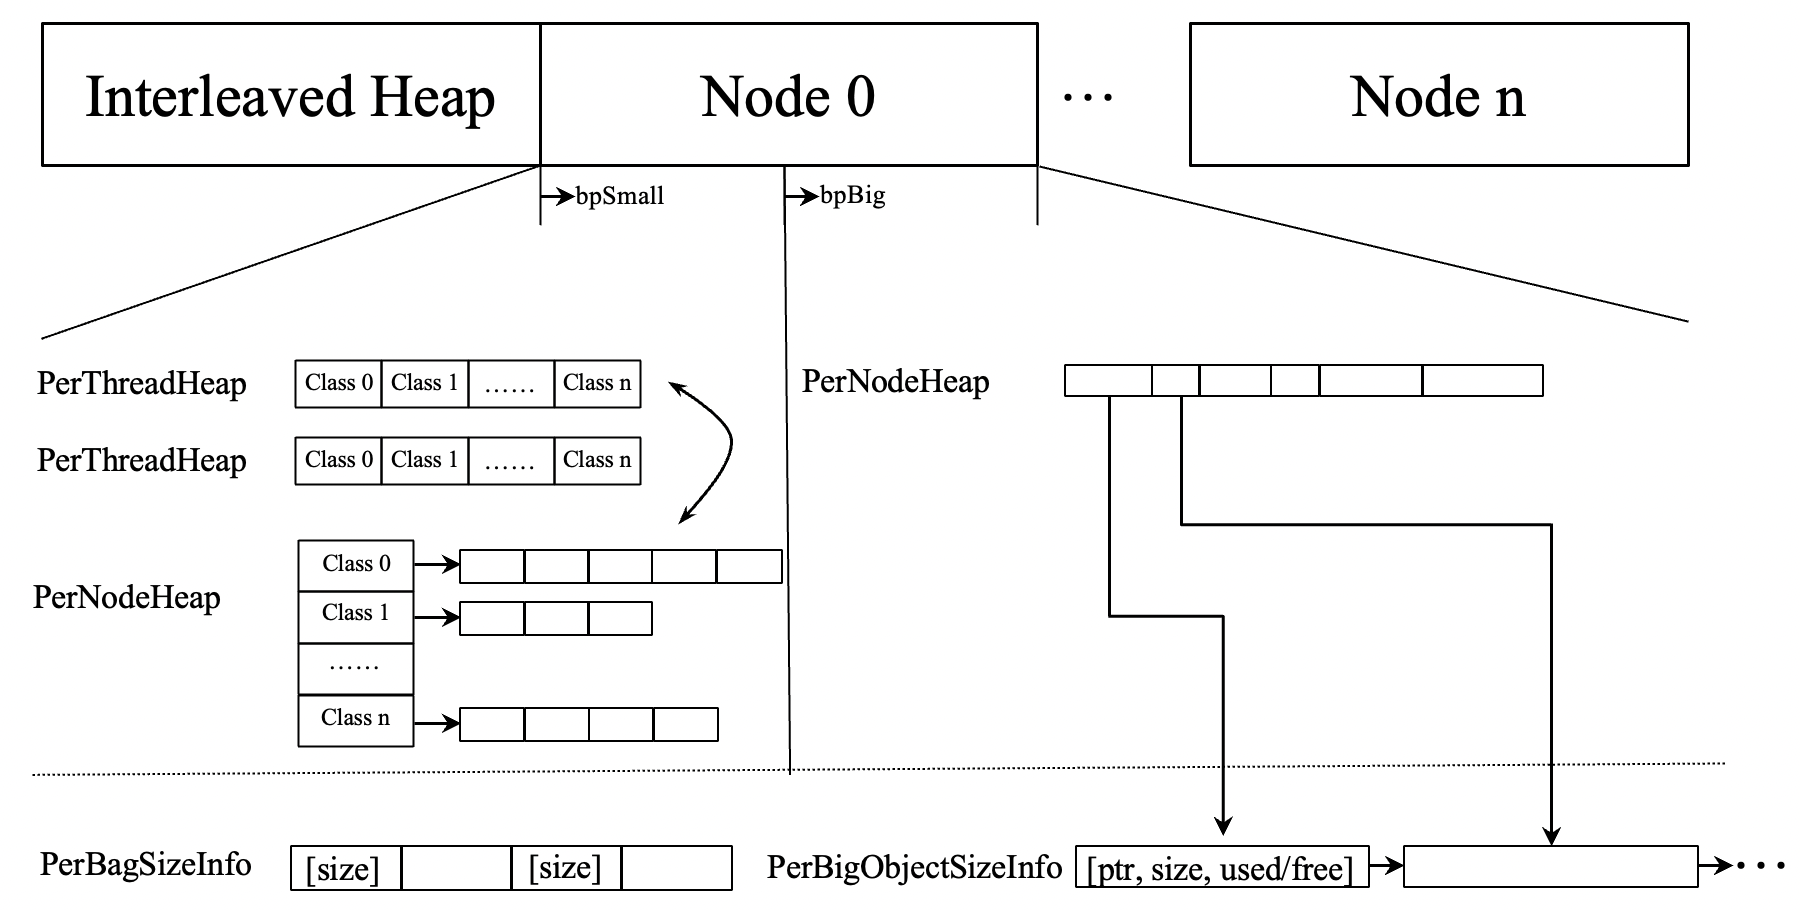
\includegraphics[width=0.45\textwidth]{SC2022/figure/numalloc-overview.png}
%\includegraphics{figure/overview2}
\end{center}
%\vspace{-0.1in}
\caption{Overview of \NA{}'s heap layout.
\label{fig:overview}}
%\vspace{-0.1in}
\end{figure}

% \todo{We should balance what to talk about in the overview, it's a little bit long and something has repeatedly described in the following}

%As discussed in Section~\ref{sec:intro}, \NM{} designs a origin-computable mechanism that could quickly check the origin of every object upon deallocation. In order to support this, 
\NM{}'s heap layout is designed as  Fig.~\ref{fig:overview}. Initially, \NM{} requests a large and continuous block of memory from the underlying OS, and then divides it evenly into multiple regions based on the number of hardware nodes. Each region is bound to a different physical node via \texttt{mbind} system call. 
%\NM{} can support the customized binding from users. If not, it typically  
In particular, the first region is bound to the first node, the second one is bound to the second node, and so on. This design enables us to compute the physical node quickly from a memory address: we could compute the index of the physical node by dividing the heap offset by the region size. 
%This layout is different from existing allocators, based on our knowledge. 
% \todo{Numalloc's reviewer said TCMalloc also use the same mechanism. I check the code and it's true that TCMalloc use the memory tag for numa partition id}
%\NM{} borrows some of these existing mechanisms. First, it uses different mechanisms to manage small and big objects. Second, small objects are also managed by size classes using the BiBOP-style. Third, similar to existing work, such as Linux and TCMalloc~\cite{tcmalloc}, \NA{} utilizes different freelists to track freed objects, and uses the first word of freed objects to link different objects. But the difference of \NM{} is further described in Section~\ref{sec:implement}.
% From Fig.~\ref{fig:overview}, we see that 
Each node's memory region will be further divided into two sub-regions, one for small objects, and the other one for big objects. The \texttt{bpSmall} pointer is utilized to track never-allocated memory
% \todo{someone doesn't understand} 
for small objects, and the \texttt{bpBig} pointer tracks the position of big objects. Similar to existing allocators, \NM{} manages small and big objects differently. 
% In \NM{}'s design, small objects are those with a size less than 512K, which are organized by size classes and each request will be satisfied from a particular size class. 
For small objects ($<$ 512KB), each request will be satisfied from a particular size class
% \NA{} utilizes fine-grained size classes, such as 16 bytes apart for objects less than 128 bytes, and 32 bytes apart for objects between 128 bytes and 256 bytes, then power-of-2 sizes afterward. 
and \NM{} utilizes the well-known ``\textbf{Bi}g-\textbf{B}ag-\textbf{o}f-\textbf{P}ages'' (BiBOP) style that all objects in the same bag (32KB by default) will have the same size class. 
Big object allocation will be satisfied in a sequential manner and their sizes are aligned to the size of one bag.

To support the NUMA architecture, a per-node heap (PerNodeHeap in Fig.~\ref{fig:overview}) is proposed that has one freelist for each size class and one common freelist for all big objects from the current node. 
%We will talk about the relationship between per-thread freelist and per-node freelist in Section~\ref{sec:origin}. 
%For small objects, freed objects of the same size class will be tracked with a freelist.
In order to reduce the contention, \NM{} adopts a per-thread heap (PerThreadHeap in Fig.~\ref{fig:overview}) that maintains a freelist for each size class, which requires no lock protection since each thread has its own per-thread heap. However, this may introduce memory blowup~\cite{Hoard} that freed objects of a per-thread heap cannot be utilized for future allocations from other threads, which will be addressed in Section~\ref{sec:others}. 
\NM{} tracks the small objects' size information in a separate area called PerBagSizeInfo, while the big objects utilize a linked list called PerBigObjectSizeInfo to store the size and availability information, which allows coalescing multiple continuous big objects into a bigger one upon deallocations.

% \NM{} tracks the size information and availability information in a separate area:  ``PerBagSizeInfo'' of Figure~\ref{fig:overview} is used for tracking the size of each size class for small objects.

%(shown as ``PerMBInfo'' of Figure~\ref{fig:overview}): it tracks the size of each size class for small objects, and the size of the big object (aligned to 1 MB) for big objects. This data structure also includes the used/free information for big objects, which allows coalescing multiple continuous big objects into a bigger object upon deallocations. To save space, \NM{} utilizes the lowest significant bit of ``PerMBInfo'' to encode the availability information.

Overall, \NM{} includes a layout that can quickly compute the physical node (with the memory binding) and a per-node heap to support node-aware allocations. This design allows it to perform incremental sharing and origin-aware memory management efficiently, as discussed in the following sections.

%mechanisms to re and one per-node freelist for each node to track big objects. \NM{} also maintains per-node freelists to track small objects based on size classes. These freelists are singly linked lists, which uses the first word of every freed object as pointers.  Small freed objects may be migrated between per-thread freelists and per-node freelists, as further described in Section~\ref{sec: others}. 
\subsection{Binding-Based Memory Management} 
\label{sec:balance}
As described in Section~\ref{sec:intro}, thread migration will cause multiple performance issues for the NUMA architecture. Therefore, \NM{} binds each thread to a node specifically to avoid thread migration across different nodes.  \NM{} currently supports two types of binding, \textbf{node-interleaved binding} and \textbf{node-saturate binding}. Node-interleaved binding binds continuous threads to different nodes in an interleaved way so that every node will have a similar number of threads. That is, the first thread will be bound to the node that it is scheduled to run by the OS, and the second thread will be bound to its next node, and so on. Instead, the node-saturate binding will bind sufficient threads to a node first before binding to a different node. For node-saturate binding, threads to be assigned will be the same as the number of hardware cores.  \NM{} will use node-interleaved binding by default, as it has a better performance based on our evaluation. But users \NEW{can} switch to the node-saturate binding by controlling the environment variable. Further, users \NEW{can} provide their customized binding via a file, which will be supported in the future. 

Note that \NM{} only binds a thread to a node, instead of a core, which still allows the scheduling initiated by the OS. To perform the binding correctly, \NM{} obtains the hardware topology in the initialization phase via the \texttt{numa\_node\_to\_cpus} API, which tells the relationship between each CPU core and each 
% memory 
node. Then it intercepts all thread creations in order to bind a newly-created thread to a specific node.

\subsection{Origin-Aware Memory Management} 
\label{sec:origin}

%\todo{In Section III-B, you talk about satisfying allocations from the "un-allocated region" as the last step. Is this memory that is not part of the interleaved heap? It would help to be more clear about what this is. }

As described in Section~\ref{sec:overview}, \NM{} includes an origin-computable design that could quickly determine the origin of each heap object via the computation. 
%On top of it, we further discuss other aspects of \NM{}'s origin-based memory management as follows.
On top of it, \NM{} proposes an origin-aware deallocation that will always return a freed object to a freelist with the same origin. In particular, if a freed object is originated from a different node, it is returned to its original node's  freelist. Otherwise, a small object is returned to the current thread's freelist and a big object is returned to the current node's freelist. Comparing to node-based freelists, there is no need to acquire a lock when operating on the per-thread freelist. Different from all existing work, \NM{} may return a freed object into the per-thread list or its original node's freelist, instead of simply putting it into the per-thread list. That is, \NM{} considers the \NEW{origination} of objects for deallocations. 

\NM{} always ensures node-local memory allocations. For small objects, it follows this order: (1) The per-thread's freelist will be checked first, since there is no need to acquire any lock and objects may be still hit in the cache (as they are just accessed by the thread). (2) If the per-thread freelist does not have available objects, \NM{} tries to allocate from the current node's freelist. As mentioned above, a node's freelist holds objects originated from this node. (3) If the previous two steps fail,  we will allocate the memory from the current node's un-allocated region, as shown by \textit{bpSmall} in Fig.~\ref{fig:overview}. 
%Since the region is bound to the current node, and objects in the per-thread freelist and the per-node freelist are always originated from the current node, 
%\NM{} ensures local allocations for small objects. 
For big objects, allocation will be satisfied from per-node freelists or un-allocated region (pointed by \textit{bpBig} pointer in Fig.~\ref{fig:overview}) of the current node, indicating the allocation locality. 
\subsection{Incremental Sharing}
\label{sec:hugepages}
When Transparent Huge Page (THP) is enabled, the OS will prefer to allocate huge pages if a program touches a continuous memory region with a size larger than a huge page (e.g., 2MB). Since \NM{} allocates a large region initially (as shown in Fig.~\ref{fig:overview}), huge pages will be employed by the OS correspondingly. However, it is important to reduce memory fragmentation, as one allocation from a memory block will be assigned to a huge page.
\NM{} makes multiple threads (from the same node) share the same huge page, instead of having a separate superblock for each thread as Scalloc~\cite{Scalloc} and TEMERAIRE~\cite{TEMERAIRE}. That is, when a thread is running out of memory, it obtains only multiple objects at a time (currently 32KB) from the corresponding memory block, instead of getting few megabytes for each per-thread heap. For small objects larger than 32KB (but less than 512KB), each thread will get only one object at a time, by aligning to 32KB as well.  This is why it is called ``incremental sharing''. 
\NM{} allocates objects with different size classes to share the same huge page, to further reduce the memory fragmentation. 

During the implementation, we observe that \NM{} actually will utilize huge pages for metadata, which may introduce unnecessary memory overhead since it only needs 8 bytes for ``PerBagSizeInfo'' used internally by \NM{}. To get rid of this overhead, we leverage the \texttt{madvise} system call to make the metadata memory allocate from normal pages. These are the basic reasons that \NM{} has much less memory consumption than Scalloc, as evaluated in Section~\ref{sec:memory}. 

\subsection{Other Mechanisms}
\label{sec:others}

\NM{} also implements the following mechanisms in order to improve the performance.



\subsubsection{Interleaved Heap} 
\NA{} proposes an interleaved heap that is inspired by existing profilers\cite{XuNuma, MemProf}: \textit{many NUMA performances issues are related to shared objects allocated in the main thread}. Due to the default first-touch policy~\cite{lameter2013numa, diener2015locality}, objects allocated and touched by the main thread are typically allocated in the node that the main thread is running on. However, these objects can be passed to multiple child threads and be accessed by these threads concurrently so that this node's memory controller becomes the performance bottleneck. 
To reduce this issue, \NA{} reserves a range of memory for such objects, called ``Interleaved Heap'' as shown in Fig.~\ref{fig:overview}. \NA{} utilizes the \texttt{mbind} system call to specify that physical pages of this heap will be allocated from all nodes interleavedly. With this design, when these objects are passed to child threads, these threads may access objects that are allocated from multiple nodes, reducing interconnect congestion and load imbalance of a single node. 
As we evaluated in Section~\ref{sec:interleavedheap}, the interleaved heap is beneficial to the performance of some applications. However, the interleaved heap will turn some of the local accesses in the serial phase into remote ones, thus degrading the performance, especially when an application spends a lot of time in its serial phase. Therefore, the interleaved heap is provided as an option that can be enabled whenever necessary. 
% However, it may degrade the performance, especially when an application spends a lot of time in its serial phase. Based on the first-touch policy, all accesses in the first serial phase for allocators using the interleaved heap will be local accesses. However, the interleaved heap will turn some of the local accesses in the serial phase into remote ones. Therefore, the interleaved heap is provided as an option that can be enabled whenever necessary. 

\begin{figure}[!h]
\centering
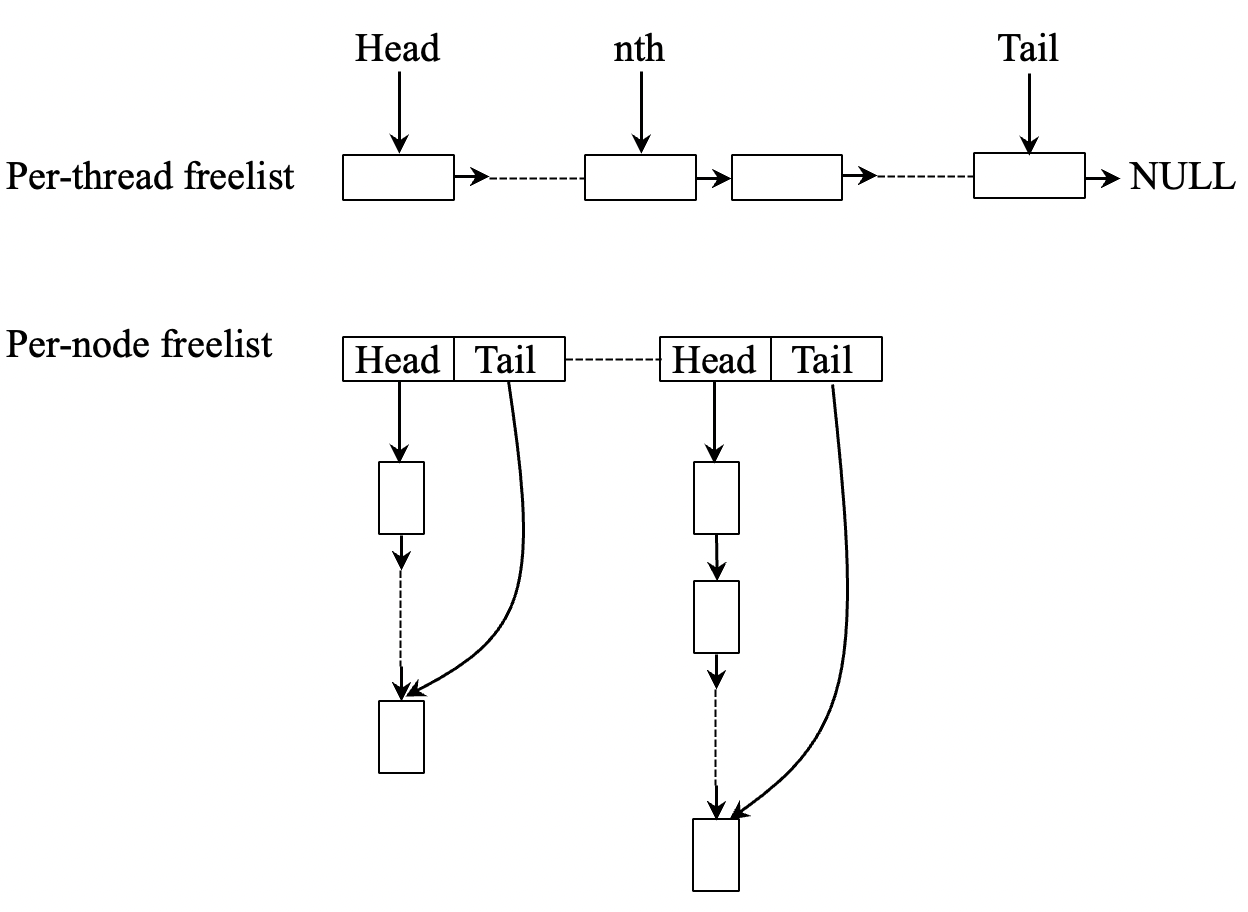
\includegraphics[width=3in]{SC2022/figure/efficient-movement.png}
%\vspace{-0.1in}
\caption{Per-thread freelist and per-node freelist design to achieve efficient object movement.\label{fig:perthreadlist}}
%\vspace{-0.1in}
\end{figure}

\begin{figure*}[!ht]
    \centering
    \includegraphics[width=7in]{SC2022/figure/8-node-parsec-perf.jpg}
    \caption{Performance of different allocators \NEW{on PARSEC and real applications}, where all data\\ is normalized to that of the default Linux allocator. Here, a lower bar indicates a better performance.
    % \todo{To adding the error-bars.}
    \label{fig:perf1}}
 \end{figure*}

\subsubsection{Efficient Object Movement} 
\label{sec:movement}
%It is important to reduce memory blowup that freed objects by one thread cannot be utilized by other threads~\cite{Hoard}. 
\NM{} requires moving freed objects between per-thread and per-node freelists frequently to reduce memory blowup. 
% An efficient mechanism is required to support the frequent movement. 
Existing allocators, such as TCMalloc~\cite{tcmalloc}, traverse the freelist to collect a specified number of objects, and then move all of them at a time, which unfortunately has the following issues: (1) traversing a freed object will bring some unnecessary data to the cache when an allocator is reusing freed objects from the freelist. This loading wastes the cache resources and evicts cache lines with useful content in the future. 
% The loading to the cache is wasted when these objects are moved to other lists later, which will evict cache lines with useful content in the future. 
(2) Existing allocators will typically move recently-freed objects (and hot in cache) to other freelist, which is not good for the performance. (3) The traverse of the shared list may introduce significant lock contention, if multiple threads are waiting to move objects from the shared list. 
\NM{} proposes an efficient mechanism with the following data structures. First, each per-thread freelist maintains two pointers that point to the least recently used objects, shown as the \texttt{Tail} pointer and the $nth$ pointer (counted from the tail) in the upper part of  Fig.~\ref{fig:perthreadlist}. 
This structure avoids the traverse of freelist during the movement, and allows the movement of the least recently used objects (between $(n+1)th$ and $Tail$) to the per-node freelist. After the movement, the \texttt{Tail} pointer will be set to the original $nth$ object. 
Second, \NM{} also proposes a circular array shown in the bottom part of Fig.~\ref{fig:perthreadlist} that helps move objects from the shared per-node  freelist to per-thread freelists. 
%As mentioned above, the per-node freelist could easily become the performance bottleneck, since multiple threads may compete for it concurrently. To address this issue, 
Each per-node freelist actually consists of many sub-lists, where a \texttt{Head} pointer and a \texttt{Tail} pointer point to the header and the tail of each sub-list. When a thread is moving multiple objects from the per-node freelist, it will move all objects in a sub-list (pointed by a pair of \texttt{Head} and \texttt{Tail} pointers) at a time. Therefore, there is no need to traverse the whole list to obtain these objects for the movement, which reduces the contention. 


%Note that this array does not increase the overhead of putting objects. If a thread puts a freed object to this array, the object can be placed into the current sub-list in a constant time. Similarly, a freelist could be appended to the current sub-list in a constant time. 



\begin{comment}
\begin{wrapfigure}{r}{0.6\textwidth}
\centering
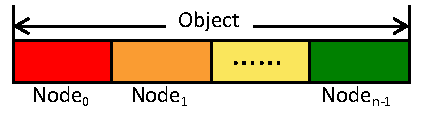
\includegraphics[width=3in]{figure/blockwise}
\vspace{-0.1in}
\caption{Block-wise Memory Allocation\label{fig:blockwise}}
\vspace{-0.1in}
\end{wrapfigure}
\end{comment}

%In theory, private objects of the first thread should not be allocated from the interleaved heap, since that will create remote accesses unnecessarily. Initially, each allocation is treated as a shared one and is allocated from the interleaved heap. Whenever a new thread is created, the allocations are regarded as private ones. Programmers can control whether they want the interleaved support or not based on their applications.


%\NM{} utilizes a simple heuristics to differentiate shared objects from private objects based on allocation callsites: each allocation callsite is treated as a shared one initially, and is allocated from the interleaved heap; Whenever an object is deallocated before creating children threads, indicating such an object is a private one for the main thread, all objects from the corresponding callsite are considered to be private ones, and they are only allocated from the per-node heap afterward. With this heuristics , there is no need to change programs explicitly, although it is more efficient if programmers could provide such information. 

% As mentioned above, \NM{} monitors the  allocation/deallocation pattern of the main thread to identify the share-ability of each callsite. 
%If an allocation callsite is found to be private, then all allocations from this callsite should not allocate from the interleaved heap, but from the normal heap. 
% A challenge is to obtain and compare the callsite of each allocation so that we could determine the heap based on the share-ability. In fact, this may introduce high overhead for applications with large amount of allocations, if using the \texttt{backtrace}~\cite{DBLP:conf/icse/SumnerZWZ10, DBLP:conf/cgo/ZengR0AJ014}. For the performance reason, \NA{} utilizes the sum of the stack position and the return address of the allocation invocation to identify a callsite, called ``\textit{callsite key}''. This combination is able to differentiate callsites correctly if an application does not have allocation wrappers, since the stack position can be utilized to identify the function in the stack and the return address tells the invocation placement inside the same function. If a callsite is misidentified, it will not cause any correctness issue, but with some performance penalties/losses. \NA{} utilizes a hash table to track the status of every callsite. 
 % which is fortunately not very expensive given the limited amount of different callsites. 
 
%Note that the interleaved heap cannot be achieved by using existing NUMA utilities like \texttt{numactl}. Although \texttt{numactl} could also specify memory allocations to be interleaved. However, \texttt{numactl} could only set the policy for a whole application. Instead, \NM{} only utilizes the interleaved heap for shared objects that are allocated in the main thread, not for all objects. 

%\todo{I remove the "Node-Local Metadata" part}

%\subsubsection{Node-Local Metadata} 
%To further reduce remote accesses, \NM{} ensures that all of the metadata is always allocated in the same node. Such metadata includes the metadata for managing per-node lists, per-thread lists, and size class information. Note that ensuring the node-local metadata for per-thread information is only possible when each thread is bound, which is the reason why \NM{} develops the ``binding-based'' approach. Therefore, \NM{} is able to guarantee that all metadata are always allocated in the same node, based on its thread binding as described in Section~\ref{sec:balance}.  
%Such metadata includes per-node and per-thread freelists for different size classes, and freelists for big objects. Similarly, \NM{} utilizes the \texttt{mbind} system call to bind the memory to a specific node.  


%Based on our evaluation, this mechanism reduces most of the memory consumption, with the transparent huge page support by default.  

 %every thread has its own freelists for each size class so that there is no need to acquire the lock when an allocation can be satisfied from its per-thread heap, similar to TCMalloc. That is, two threads will not share the same per-thread heap. However, some applications may create new threads after some threads have exited. \NM{} re-utilizes the memory for these exited threads. Basically, \NM{} intercepts thread joins and cancels so that it can assign heaps of exited threads for newly-created threads, and re-utilize their heaps correspondingly.  


%\paragraph{Transparent Huge Page Support:} During the development, we noticed that excessive memory consumption can be imposed when the OS enables transparent huge pages by default. In order to reduce memory consumption, \NM{} makes multiple threads share the same bag (for the same size class), instead of having a separate bag for each thread. If each thread is running out of the memory, it obtains multiple objects at a time from the corresponding bag. Currently, if a class size is less than one page, then we will at most get objects with the total size of one normal page. Otherwise, it will get 4 objects (with the size less than 64 KB) or 2 objects afterward. Based on our evaluation, this mechanism actually reduces the memory consumption for multiple times for a machine with 128 cores and 8 nodes, with the transparent huge page support by default.  

%\paragraph{Cache Warmup} \NM{} also borrows the cache warmup mechanism of TCMalloc~\cite{tcmalloc}: it will insert all objects in a page into the freelists, if there is no objects in the per-thread freelist. We believe that inserting multiple objects into the freelist will benefit data prefetches, since the insertion is a simple and predictable pattern. With this mechanism, \texttt{raytrace} improves the performance by 10\%. However, this is the only application that we observed such performance improvement. There is no impact on other applications. 

%TCMalloc utilizes a \texttt{mmap} system call to obtain multiple pages (depending on the class size) from the OS each time, when it is running out of the memory for one size class. For such a memory block, TCMalloc inserts all objects of this block into its central freelist at one time. Since TCMalloc utilizes the first word of each object as the pointer for the freelist, this mechanism warms up the cache by referencing the first word of each object during the insertion. According to our observation, this warmup mechanism improves the performance of one application (\texttt{raytrace}) by 10\%. Based on our understanding, the performance improvement is caused by data prefetches, since inserting objects to the freelist has a simple and predictable pattern. \NM{} employs a similar mechanism for small objects with the size less than 256 bytes, and adds all objects inside a page to the per-thread freelist. 

%we propose the combination of per-node heap and per-thread cache. In order to reduce the contention, \NM{} will obtain multiple objects at a time from the per-node heap. 

 
%https://queue.acm.org/detail.cfm?id=2852078
 

\section{Experimental Evaluation}
\label{sec:evaluation}

This section aims to answer the following research questions: 

\begin{itemize}
\item \textbf{Performance:} How is \NM{}'s performance, comparing to existing general allocators and NUMA-aware allocators? (Section~\ref{sec:performance}) 
\item \textbf{Memory Consumption:} What is the memory consumption of \NM{}? (Section~\ref{sec:memory})
\item \textbf{Scalability:} How is the scalability of \NM{}? (Section~\ref{sec:scale})
\item \textbf{Impact of Design Choices:} \NEW{What is the impact of each design choice on} the performance of \NM{}? (Section~\ref{sec:design})	
\end{itemize}



\begin{comment}

\begin{table}[!ht]
 \centering
   \caption{Machine specifications for evaluation
   \label{table:Machine}}
  %\setlength{\tabcolsep}{1.0em}
\begin{tabular}{l | l }
\hline
Category & Information \\ \hline
CPUs/Model 	& Xeon(R) Platinum 8153\\ \hline
CPU Frequency & 2.00GHz\\ \hline
NUMA Nodes  & 8 \\ \hline
Physical Cores  & 8$\times$16 \\ \hline
Node Latency &  \specialcell{local: 1.0 \\ 1 hop: 2.1 \\ 2 hops: 3.1}\\ \hline
Interconnect Bandwidth  & 10.4GT/s\\ \hline
Linux & Debian 10\\ \hline
Compiler &  GCC-8.3.0 \\ \hline
%Memory Bandwidth & 19.87 GB/s & \\ \hline
  \end{tabular}
  %\vspace{-0.4in}
\end{table}
\end{comment}

\textbf{Experimental Setup:}  \NM{} was evaluated on an Intel Xeon(R) Platinum 8153 machine with 8 nodes, where each node has 16 cores.  \NEW{8 nodes are divided into two groups, where the four nodes of each group are fully connected, and there are four links between the two groups. Any two nodes are less than or equal to 2 hops, where the latency of one hop and two hops is 2.1 and 3.1 separately if the latency of local accesses is 1.0}. The machine is installed with 512GB memory. \NEW{Each core has a dedicated L1 (32KB) and L2 (1MB) cache, and cores within a node share a 22MB last-level cache (LLC).} The underlying OS is Linux Debian 10 and the compiler is GCC-8.3.0. In the evaluation, the hyperthreading was turned off, but both transparent huge page and AutoNUMA are enabled. We utilize 128 threads, which is the same as the number of cores of the evaluated machine. \NEW{For OpenMP/MPI applications, we use a hybird MPI + OpenMP mode where the number of MPI processes is equal to the number of nodes and each process has 16 OpenMP threads which is the core number inside a processor.} The performance data shown in this paper is an average of 30 executions, in order to avoid any bias caused by unexpected events.

% \todo{Adding the hardware issue, about node, about LLC} 
% \todo{Adding the glibc's version}

\textbf{Compared Allocators and Evaluated Applications: }  We compare \NM{} with multiple popular allocators, such as the default Linux allocator \NEW{(Glibc-2.28)}~\cite{glibcweb}, TCMalloc~\cite{tcmalloc2},  TCMalloc-NUMA~\cite{tcmallocnuma}, jemalloc-5.2.1~\cite{jemalloc}, Intel TBB-2021.5~\cite{tbb2}, Scalloc-1.0.0~\cite{Scalloc}, and mimalloc\NEW{-1.6.7}~\cite{mimalloc}. Note that we are comparing against TCMalloc's NUMA awareness version (released in July 2021), and the newest version of TBB with NUMA support (released in December 2021). Note that the evaluated TCMalloc already includes TEMERAIRE~\cite{TEMERAIRE}'s huge page support. 
%Among them, TCMalloc, jemalloc, TBB, and mimalloc are commercial allocators designed and maintained by Industrial Giants, like Google, Facebook, Intel, and Microsoft separately. 
We do not include Hoard~\cite{Hoard} as it is not the state-of-art anymore~\cite{Scalloc, mimalloc}. Multithreaded applications chosen to evaluate the performance include PARSEC applications~\cite{parsec}, \NEW{five OpenMP/MPI applications from CORAL-2 Benchmarks~\cite{coral2}, including \texttt{Nekbone}, \texttt{QMCPACK}, \texttt{LAMMPS}, \texttt{AMG} and \texttt{Quicksilver}}, and real applications such as \texttt{Apache httpd-2.4.35}, \texttt{MySQL-5.7.15}, \texttt{Memcached-1.4.25}, \texttt{SQLite-3.12.0}, \texttt{Aget}, \texttt{Pfscan} and \texttt{Pbzip2}.

%Note that we currently have an issue running freqmine, an openmp application, which is excluded right now. 

 \begin{figure}[!h]
    \centering
    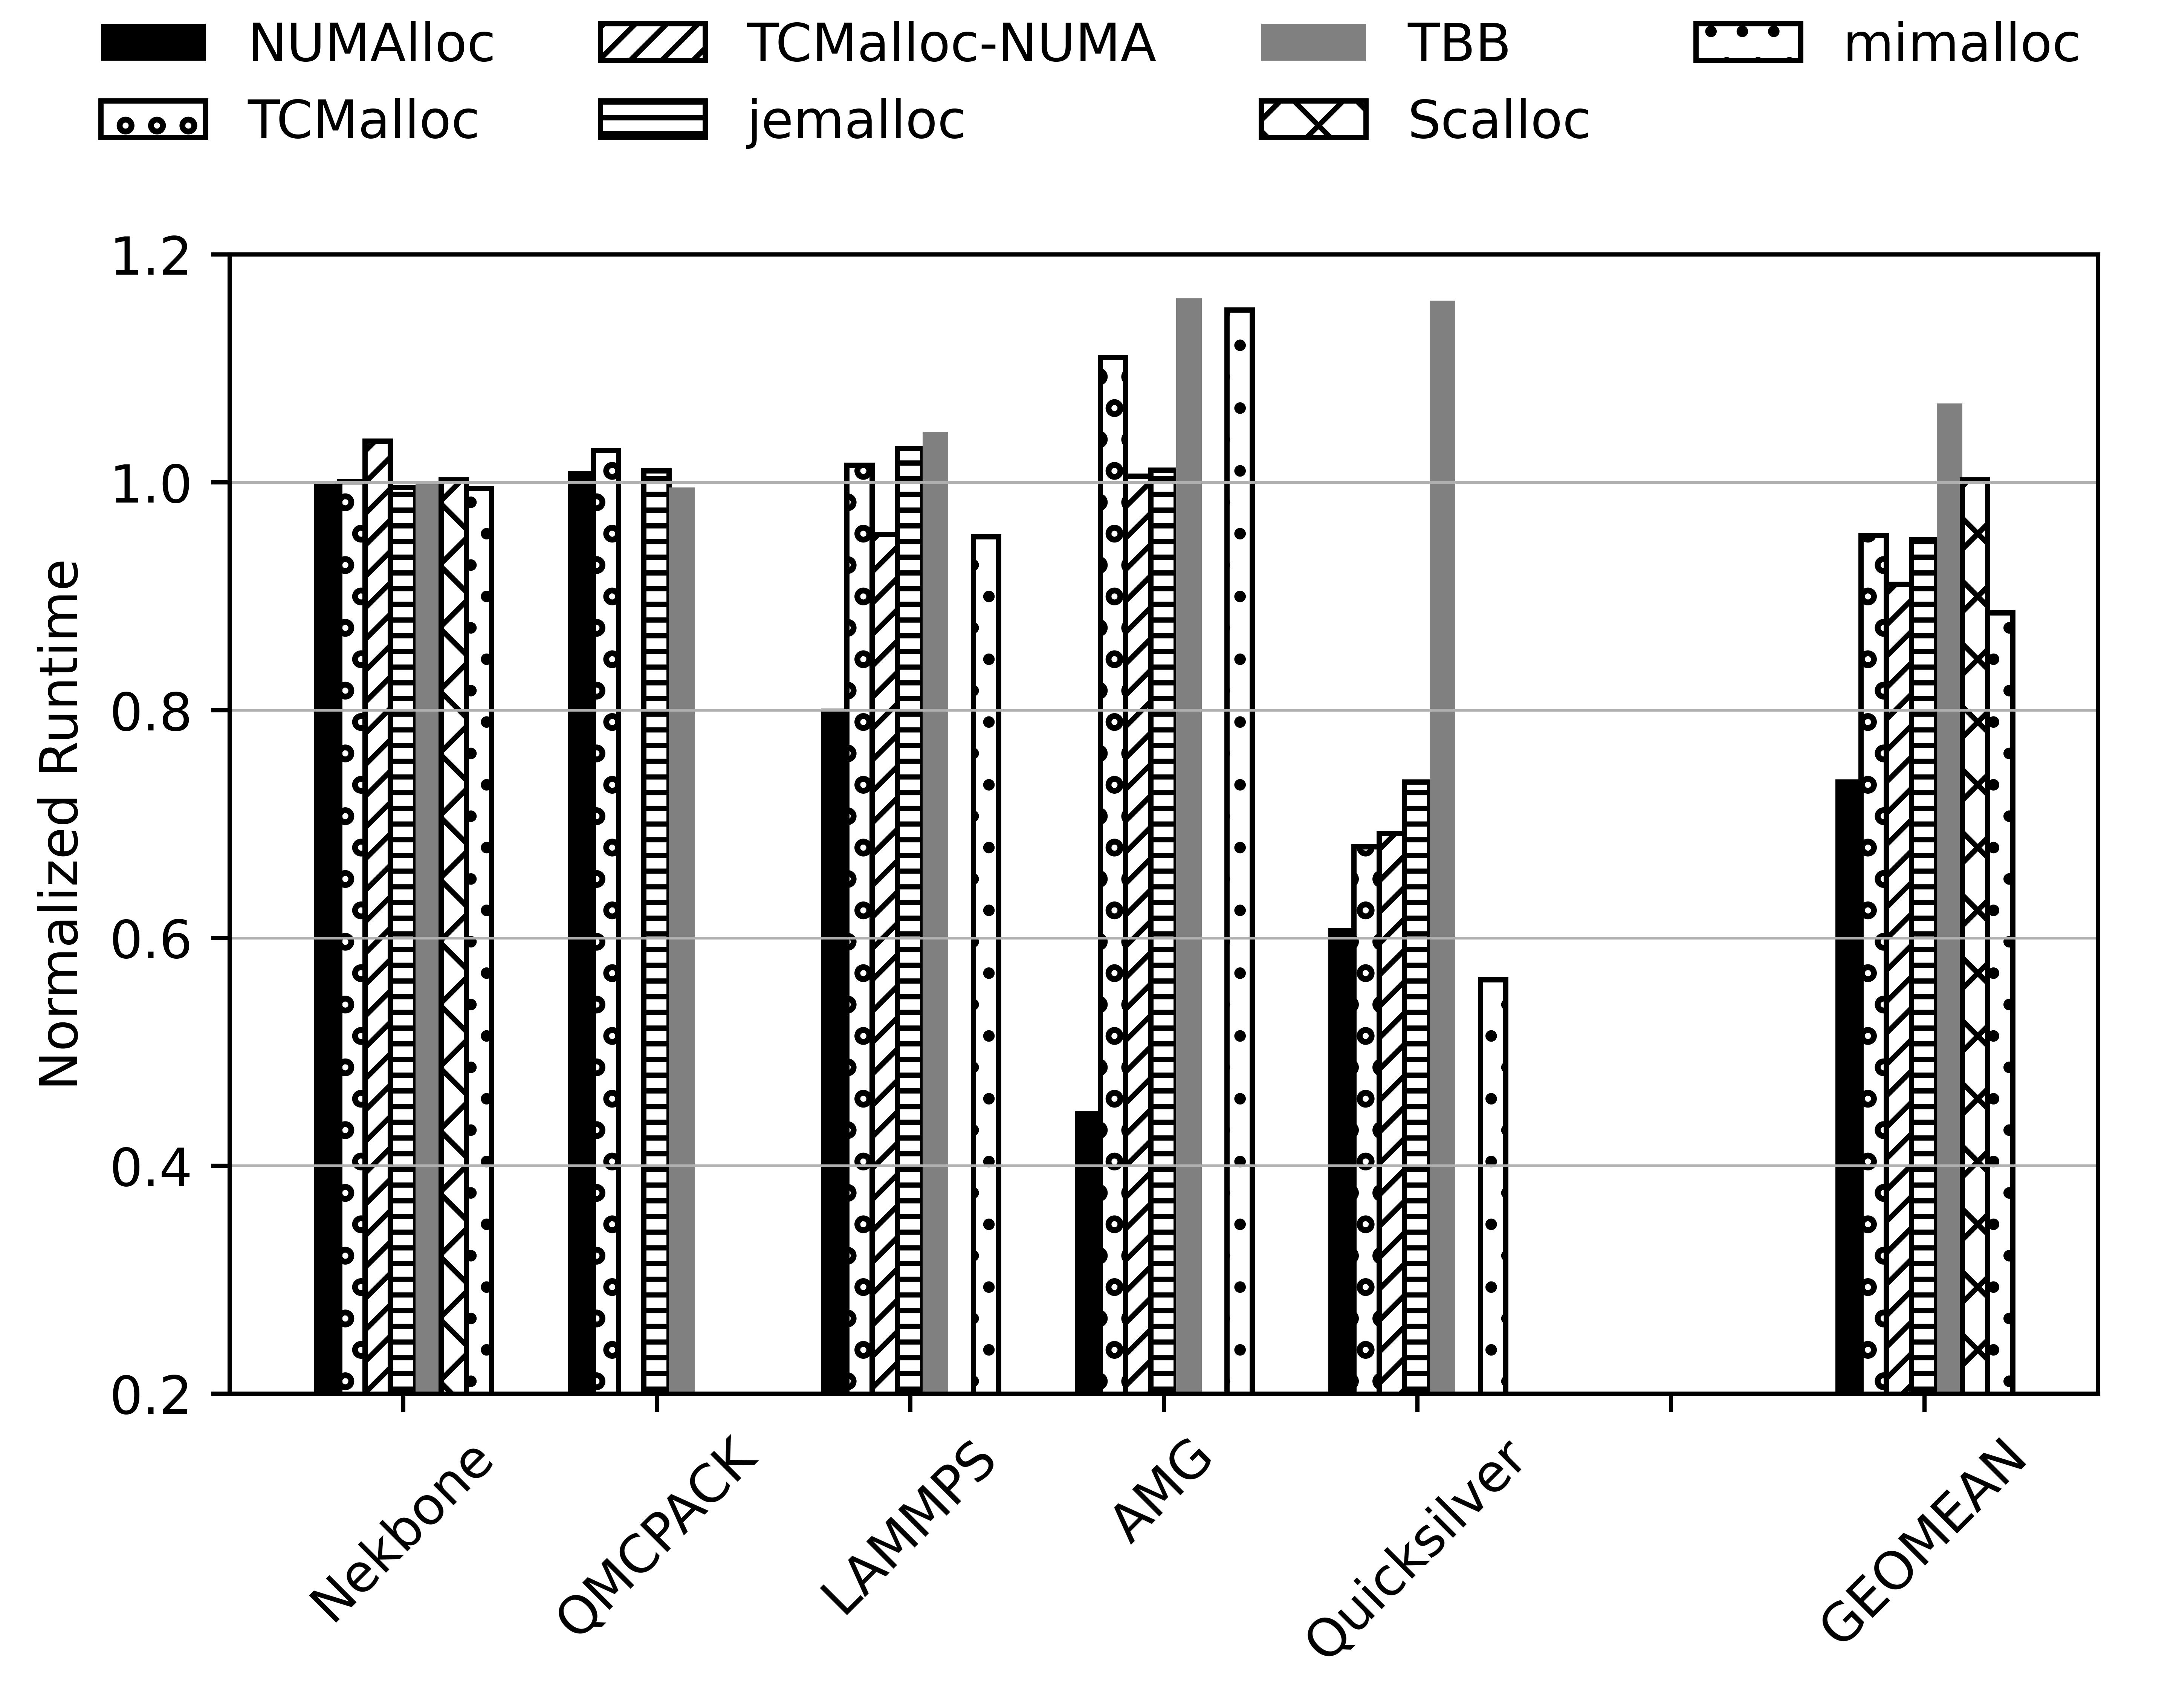
\includegraphics[width=3.5in]{SC2022/figure/8-node-mpi-perf.jpg}
    \caption{\NEW{Performance of different allocators on OpenMP/MPI applications, where all data is normalized to that of the default Linux allocator. Note that some applications are failed to run with some allocators.}
    \label{fig:perf2}}
 \end{figure}

\begin{comment}
\begin{table}[!ht]
 \centering
  %\setlength{\tabcolsep}{1.0em}
\begin{tabular}{c | c | c}
\hline
System & \textbf{Machine A} & \textbf{Machine B} \\ \hline
CPUs/Model & Xeon Gold 6138	& Xeon(R) Platinum 8153\\ \hline
CPU Frequency & 2.10GHz & 2.00GHz\\ \hline
NUMA Nodes & 2 & 8 \\ \hline
Physical Cores & 2$\times$20 & 8$\times$16 \\ \hline
Node Latency & \specialcell{local: 1.0 \\ 1 hop: 2.1} & \specialcell{local: 1.0 \\ 1 hop: 2.1 \\ 2 hops: 3.1}\\ \hline
Interconnect Bandwidth & 8GT/s & 10.4GT/s\\ \hline
Linux & Ubuntu 18.04 & Debian 10\\ \hline
Compiler & GCC-7.5.0 & GCC-8.3.0 \\ \hline
%Memory Bandwidth & 19.87 GB/s & \\ \hline
  \end{tabular}
   \caption{Machine specifications for evaluation
   \label{table:Machine}}
  %\vspace{-0.4in}
\end{table}
\end{comment}

\subsection{Performance Evaluation}
\label{sec:performance}

% PARSEC applications are using native inputs~\cite{parsec}. For \texttt{MySQL}, we use \texttt{sysbench} with 128 threads separately, each issuing 100,000 requests. The \texttt{python-memcached}  is used to exercise \texttt{Memcached}, with 3000 loops to get the sufficient runtime~\cite{memcached}. The \texttt{ab} is used to test \texttt{Apache} server~\cite{apachetest}, by sending 1,000,000 requests in total. \texttt{Aget} is tested by downloading a 30-MB file, and \texttt{Pfscan} is tested by searching  a keyword in a 500MB data. In terms of \texttt{Pbzip2}, we test it by compressing 10 files with 30MB each. Finally, \texttt{SQLite} is tested through a program called \texttt{threadtest3}~\cite{sqlitetest}. 

%\todo{The number of threads of all benchmarks were adjusted according how many cores and nodes in the target machine to make threads could be properly distributed over the nodes and cores, making the number of threads as close as the number of cores. In the test machine, the thread number is 128.}

%In the Hoard~\cite{Hoard} benchmarks, we used 100 iterations and 1,280,000 64-byte objects for threadtest and also we run larson for 10 seconds with 1,000 7-2048 bytes object to cover all size classes in almost all allocators for 10,000 iterations.For false sharing , we used 100,000 inner-loop , 100,000 iterations with 8 bytes objects. 

%The number of threads of all benchmarks were adjusted according how many cores and nodes in the target machine to make threads could be properly distributed over the nodes and cores, making the number of threads as close as the number of cores. Mostly, thread number was 40 in the Machine A and 128 in the Machine B, and I will give the specific number below if it is not this default value. 

The performance results are shown in Fig.~\ref{fig:perf1} and Fig.~\ref{fig:perf2}, where the runtime of each allocator is normalized to that of Linux's default one. \NM{} is configured without the interleaved heap support for most applications, except for \texttt{fluidanimate} and \texttt{streamcluster}. As evaluated in Section~\ref{sec:interleavedheap}, the interleaved heap will significantly improve the performance for these two applications. 
%As further discussed in Section~\ref{sec:interleavedheap}, the interleaved heap may have a harmful performance impact for the serial phases, as it turns some local accesses to remote ones. %Therefore, the data of \texttt{canneal} and \texttt{raytrace} are collected without the interleaved heap. 
%We believe that this option is acceptable, since users could determine easily whether they should disable the interleaved heap: if an application has a large portion in the serial phase, then the interleaved heap should be disabled. 
%The impact of the interleaved heap is further discussed and evaluated in Section~\ref{sec:interleavedheap}. 
 %With the interleaved heap,  allocations from the main thread can be satisfied in remote NUMA nodes, this design may lead to a large number of remote accesses for the serial phase. since both of them spend a large portion of their time (over 62\% and 82\%) in the serial phase (before creating any child thread),
 %These two figures show the best data for these two applications, without the support of the interleaved heap.    
Overall, \NM{} has the best performance among these allocators. In particular, \NM{} is \NEW{15.7\%} faster than the second-best allocator (mimalloc) and \NEW{19.0\%} faster than the default Linux allocator. %\todo{explain why mimalloc is good? why other allocators are not good}
For the best case (e.g., \texttt{fluidanimate}), \NM{} is running up to $5.3\times$ faster than the default Linux allocator, and $6.8\times$ faster than Scalloc.
On average, \NM{} is \NEW{18.2\%}, \NEW{16.3\%}, and \NEW{18.8\%} faster than TCMalloc~\cite{tcmalloc2}, TCMalloc-NUMA~\cite{tcmallocnuma}, Intel TBB~\cite{tbb3}. \NEW{Considering only OpenMP/MPI applications, applications run 26.1\% faster with \NM{} compared with the default Linux allocator, and 16.5\% faster than the second-best allocator (mimalloc).}

\begin{figure}[!h]
    \centering 
    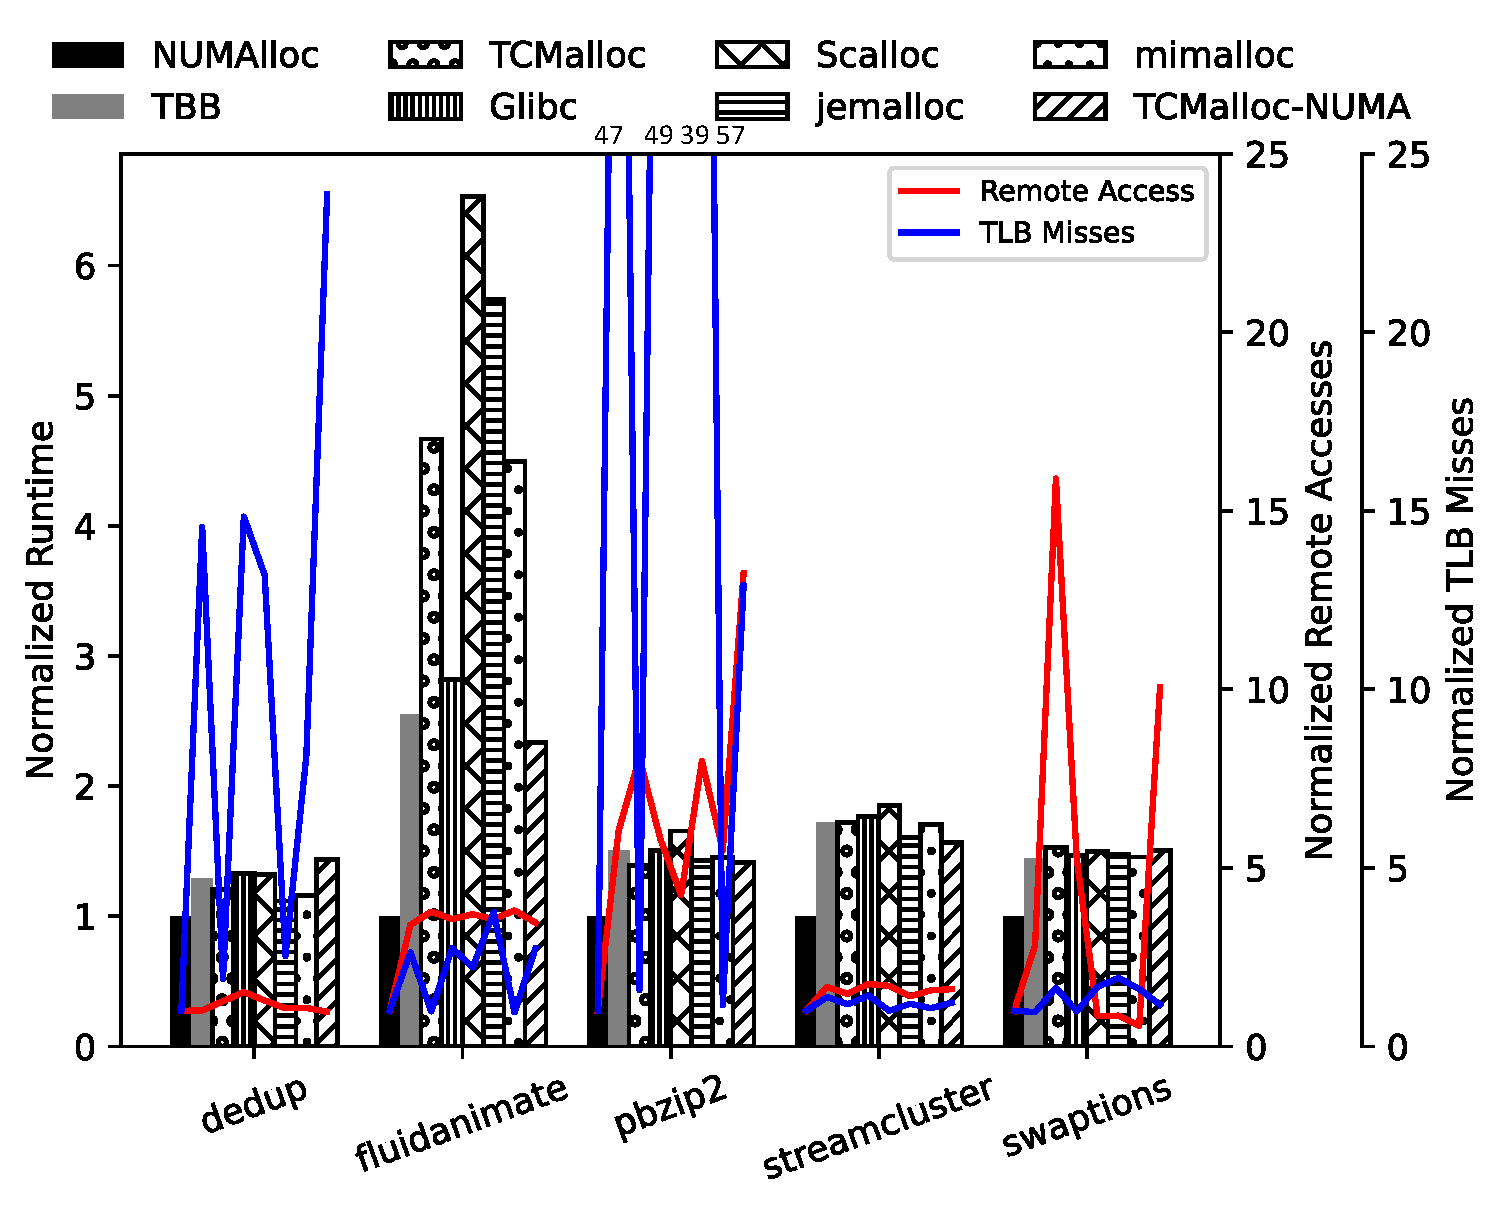
\includegraphics[width=3.5in]{SC2022/figure/remote access.pdf}
    \caption{Normalized runtime, remote accesses, and TLB misses of different allocators (to \NM{}), where the lower is the better. }
    \label{fig:remoteAccess}
\end{figure}

%\NM{} is running \todo{19\%} faster than the default allocator, but does not run significantly slower than other allocators in almost all evaluated applications. For the best case (e.g., \texttt{fluidanimate}), \NM{} is running up to \todo{$6.4\times$} faster than the default Linux allocator.
%The default Linux allocator achieves good performance on the NUMA architecture due to its arena-based design, where each freed object will be returned back to its original arena. This design is integrating well with Linux's first-touch allocation policy~\cite{Lameter:2013:NO:2508834.2513149} to ensure most thread-local allocations. 
% In contrast, other allocators typically utilize a per-thread cache to store objects that are deallocated by the current thread, which may lead to remote accesses as described in Section~\ref{sec:intro}.
% Comparing with the NUMA-aware allocator -- TCMalloc-NUMA~\cite{tcmallocnew}, \NM{} runs \todo{23\%} faster. 
%TCMalloc-NUMA, TCMalloc, TBB, and mimalloc are allocators that are claimed to support the NUMA architecture~\cite{tcmallocnew}. 
%But TCMalloc-NUMA's performance is even worse than that of TCMalloc. Based on our understanding, TCMalloc-NUMA is based on TCMalloc-0.97 (released in 2008), which does not have new features of TCMalloc-2.7 (the version for our evaluation). 
% mimalloc only has the very basic NUMA support, which is the reason why it is not performing as well as \NM{}. TCMalloc and TBB are allocators that are claimed to support the NUMA architecture~\cite{tcmalloc2, tbb3}, but \NM{} is \todo{21\%} faster than both of them.

As shown in Fig.~\ref{fig:perf1}, \NM{} has a significant performance improvement (over 25\%) in the following applications, including \texttt{dedup}, \texttt{fluidanimate}, \texttt{pbzip2}, \texttt{streamcluster}, and \texttt{swaptions}. For these applications, we further examine the number of remote accesses and TLB misses to confirm whether \NM{} significantly reduces them. 
% By ensuring the full locality of memory accesses, \NM{} is expected to reduce the number of remote accesses. \NM{} will reduce the TLB misses, since it takes the advantage of transparent huge pages.  
We utilize the \texttt{perf}\NEW{~\cite{perfweb} (version 4.19), a Linux performance profiling tool,} to collect these numbers. 
% Figure~\ref{fig:perf} shows that \NM{} has a similar or better performance than the default allocator in almost all applications. Further, it has a significant performance improvement (over 20\%) in the following applications, including \texttt{canneal}, \texttt{dedup}, \texttt{fluidanimate}, \texttt{streamcluster}, and \texttt{pbzip2}. Among them, \NM{} has a better performance for \texttt{fluidanimate}, due to the following reasons. First, the interleaved heap contributes to $3.23\times$ performance speedup, as shown in Figure~\ref{fig:interleavedheap}. Second, node-balanced thread binding improves the performance by over $4\times$. 
% \textbf{Confirming the number of remote accesses:} We further examine the number of remote accesses to confirm whether \NM{} significantly reduces them due to its design. We utilize the \texttt{perf} to collect the number of remote accesses (both load and store) on these applications when they are running with all allocators. 
%In our machine, we can collect these numbers using the following command: \texttt{perf stat -e node-load-misses,node-store-misses,dTLB-store-misses,dTLB-load-misses} 
The results are shown in Fig.~\ref{fig:remoteAccess}, which includes the performance (shown as bars), remote accesses (red lines), and TLB misses (blue lines) together for a better comparison. 
% For all these data, the lower is better. 
Overall, \NM{} has either a lower number of remote accesses or TLB misses than other allocators, which explains why \NM{} is the fastest on these applications. We also notice that both \NM{} and TCMalloc have a lower number of TLB misses, as they have the support for huge pages.   

%We only use five applications that \NM{} has significantly better performance than other allocators.
\NM{} significantly reduces the number of remote accesses for three applications, \texttt{fluidanimate}, \texttt{pbzip2}, and \texttt{streamcluster}. Let us utilize \texttt{fluidanimate} as an example, where \NM{} is running $2.9\times$ faster than the default Linux allocator and $4.6\times$ faster than TCMalloc. Fig.~\ref{fig:remoteAccess} shows that the number of remote accesses for the default allocator and TCMalloc is $3.6\times$ and $3.8\times$ more than \NM{}. However, there is no much difference in the number of remote accesses for \texttt{dedup} and \texttt{swaptions} compared with some allocators. Based on our investigation, \NM{} is running faster than others due to the reduction of TLB misses instead. 
\NEW{We also conduct such experiments on the OpenMP/MPI applications shown in Fig.~\ref{fig:perf2}. Compared with the second-best allocator (mimalloc), the remote accesses of \NM{} are reduced by $13.9\times$ and the TLB misses are reduced by $1.08\times$ on average. The data for other allocators are similar or even worse. This further confirms that \NM{} can reduce the number of remote accesses as well as TLB misses, thus improving the performance.}

\NM{}'s big reduction of remote accesses can be attributed to the following factors: its thread binding avoids unnecessary remote accesses; its metadata is placed on the local node, based on the binding design; its origin-aware memory allocation ensures locality of memory allocations.
For TLB misses, \NM{} is orders of magnitude lower than other allocators (except TCMalloc) for \texttt{pbzip2}. Especially, the default allocator and jemalloc have $48\times$ or $57\times$ more TLB misses. Interestingly, the performance difference of \texttt{pbzip2} is even smaller than \texttt{fluidanimate}, given the large difference in TLB misses. Based on our understanding, \texttt{pbzip2} is an IO-bound application so that the computation difference does not have a large impact on its overall performance. 
%\NM{} has a  more close to those of other allocators for \texttt{swaptions}.
Overall, \NM{} either has fewer remote accesses or fewer TLB misses, which \NEW{are the reasons that \NM{} has} better performance than other allocators on these applications. 

%\renewcommand{\arraystretch}{1.5}
\begin{table}[tp]
\footnotesize
	\setlength{\tabcolsep}{0.3em}
  \centering
    \begin{tabular}{|l|r|r|r|r|r|r|r|}
    \hline
    \multirow{2}{*}{Apps}&
    \multicolumn{7}{c|}{Memory Usage (MB)}\\
    \cline{2-8}
    &Linux&\NM{}&TcM&TcM-N&jem&TBB&Scalloc \\ \hline
    \hline
    blackscholes&615&509&621&623&633&615&630\\ \hline
    bodytrack&37&161&45&46&570&37&1994\\ \hline
    canneal&888&879&774&757&1294&888&36149\\ \hline
    dedup&912&1236&983&1023&1389&912&8556\\ \hline
    facesim&560&500&603&601&1133&547&3056\\ \hline
    ferret&184&493&195&183&596&184&3377\\ \hline
    fluidanimate&470&392&483&484&481&470&3437\\ \hline
    raytrace&1288&1472&1092&1543&1287&1288&4398\\ \hline
    streamcluster&113&105&123&121&127&113&193\\ \hline
    swaptions&33&268&16&21&540&37&1817\\ \hline
    vips&228&536&248&269&778&227&3681\\ \hline
    x264&2859&2721&3047&3064&3719&2859&5402\\ \hline \hline  
    Aget&8&74&11&10&93&8&80 \\ \hline
    Apache&8&34&10&9&10&4&42\\ \hline
    Memcached&16&80&25&24&41&18&263\\ \hline
    Mysql&277&732&314&315&500&276& N/A \\ \hline
    Pbzip2&463&747&817&813&1121&454&4881 \\ \hline
    Pfscan&522&542&528&528&535&522&554\\ \hline
    Sqlite3&45&284&60&75&139&44&681 \\ \hline
    \hline
    Total&{\bf 9527}&{\bf 11763}&{\bf 9993}&{\bf 10510}&{\bf 14986}&{\bf 9502}&{\bf 79190}\cr\hline
    \end{tabular}
  \caption{Memory consumption of different allocators. Here, TcM stands for TcMalloc, TcM-N is TcMalloc-NUMA, and jem is jemalloc. \label{tab:memory_consumption}}
\end{table}


To further validate the effectiveness of \NM{}, we also evaluate it on the Rodinia OpenMP benchmark suite~\cite{che2009rodinia}. According to the results, applications using \NM{} gain an average speedup of $2.33\times$ compared to the second-best allocator (mimalloc), and $2.44\times$ speedup compared to the default Linux allocator, which indicates that \NM{} also performs well on OpenMP applications. Due to the page limit, we do not show the runtime of each application in this paper. 

%However, there is no much difference in the number of remote accesses for \texttt{dedup} and \texttt{swaptions} compared with some allocators.  When transparent huge page support is enabled, \NM{} utilizes huge pages instead of small pages, leading to fewer TLB misses. For example, for \texttt{dedup}, \NM{}'s TLB misses is $2.82\times$ lower than that of TCMalloc-NUMA, under the similar number of remote accesses.

% \todo{check if there is a true causality between the amount of reduced remote access and the amount of performance improvement; Better insight into some of the experiments to understand why in about 40\% of the cases NUMAlloc doesn't clearly beat other allocators.}




%For TLB misses, typically both both \NM{} and TCMalloc have lower TLB misses than others, as they all take advantage of huge pages. For \texttt{pbzip2}, other allocators (e.g., TBB, glibc, Scalloc, and jemalloc) could be dozens of larger than \NM{}'s. \todo{We can also observe this trend in \texttt{dedup} application.}

% \NM{} also has much less TLB misses on \texttt{dedup} application.

%data in https://docs.google.com/spreadsheets/d/1WqWH5J7CcQuV8Vs4HnqRSC7TZpgQGPB9Gh2knHPSZPU/edit?usp=sharing
%We also observe some similar results for other applications. For \texttt{dedup}, the \texttt{glibc} allocator introduces 17850 time more TLB misses than \NM{}. Note that we only collect these two factors here, where the performance of allocators can be caused by other reasons, such as memory management operations.

%Further, \NM{} allocates a large chunk of memory initially, then the OS tends to utilize huge pages if possible, although this mechanism may introduce more memory consumption as evaluated in Section~\ref{sec:memory}.  


%\todo{Change "Performance" to runtime, also change the the performance/remote accesses" scale to 8, maybe put NUMAlloc to the first, change TcMalloc to TCMalloc. }

\begin{comment}
\begin{table}[htp]
    \centering
    \footnotesize
    \begin{tabular}{l|c| c|c|c|c|c|c|c|c}
    \multicolumn{2}{c|}{Application} & glibc & \NM{} & TCM & TCM-NUMA & jemalloc & TBB & Scalloc & mimalloc \\ \hline
    \multirow{2}{*}{canneal} & Remote & 772 & 613 & 718   & 626 & 690 & 752 & 655 & 709\\ \cline{2-10}
    & TLB Misses &  & 975  &    &  &1876  & 1910 & 1836 & 1876 \\ \hline
    \multirow{2}{*}{dedup}  & Remote & 35.7 & 23.8 & 23.2 & 32.6 & & 29.9 & 28.4 & 23.7\\ \cline{2-10}
     & TLB &  & 21.6 &    &  & & 31.1 & 42.0  & 19.2\\ \hline
    \multirow{2}{*}{fluidanimate} & Remote  & 784 & 145 & 755 & 902 & & 741 & 798 & 749\\ \cline{2-10}
    5.2
   & TLB  &  & 11.9  &    &  & & 116 & 137 & 100\\ \hline
    \multirow{2}{*}{streamcluster} & Remote  & 762 & 571 & 602 & 548 & & 768 & 497 & 570\\ \cline{2-10}
    &  TLB  &  & 12.1 &    &  & & 1455 & 1410 &  1432\\ \hline
    \multirow{2}{*}{pbzip2} & Remote  &  59.3 & 15.2 & 102 & 98.8 & & 62.5 & 45.8 & 60.4\\ \cline{2-10}
    & TLB &  & 0.8 &    &  & & 98.1 & 66.8 & 26.7 \\ \hline
    \end{tabular}
    \caption{TLB misses when using different allocators. The data shown is mega. }
    \label{tab:characteristics}
\end{table}

\end{comment}

%Table~\ref{tab:characteristics} shows that \NM{} significantly reduces the number of remote accesses and TLB misses due to its region-based design. 

%\todo{Hanmei: maybe we need to get the data on these applications. perf stat -e node-loads, node-load-misses, node-stores, node-store-misses ./APP a.out}



%We  can see that the average value of \NM{} is 0.97 in Machine A and 0.92 in Machine B and it is always the best among all other allocators. The reason that \NM{} got better performance in Machine B is that there are more nodes and more cores in Machine B, which means \NM{} could be very helpful to better to take use hardware resource of multi nodes and cores. but we could get amazing improvement if we shutdown interleaved heap in \NM{} and we will give the data in following sections.In the figure ~\ref{8node-parsec-perf}, we could see more exciting improvement from \NM{}, with average normalized value of 0.92 that is not only the best but also far aware better than all the rest allocators that TCMalloc and jemalloc got 0.99, TCMalloc-NUMA and TBB got roughly 1.07 and 1.01 separately. And also, we can see that the performance of \NM{} is the best for almost each single applications, especially it got 0.17 in fluidanimate and 0.66 in streamcluster which is far better than any of other allocators. As the same thing, the performance of ratrace and canneal is not good here, we will talk about it later after we shut down the interleaved heap.


%In the figure ~\ref{hoard-perf}, we show the normalized performance for Hoard benchmarks in Machine A and Machine B separately. We can see from figure ~\ref{hoard-perf} that the average value of \NM{} is also the best, which is 0.47 that means 2 times faster than default Linux Allocator, and jemalloc got 0.7 and Scalloc got 0.9. In the threadtest, the normalized value of \NM{} is 0.19 , far better than any of others, which means there are few central free list competitions, mainly contributed by properly node management and low overheads operations. For false sharing, \NM{}'s performance is also almost the best as same as Scalloc and jemalloc, which means they could handle false sharing issues very properly. In the larson, \NM{} and TCMalloc are the best, which mainly contributed by their low overheads for allocation and remote de-allocation, but due to our better node management, \NM{} could be better in the Machine B which will be mentioned later. In the figure ~\ref{hoard-perf}, we can also see that \NM{} got lowest average normalized value:0.33, significantly smaller than any of others that TBB got 0.99, Scalloc and jemalloc got roughly 1.14. And also, \NM{} and Scalloc could handle false sharing issue very well, and \NM{} could extremely well reduce central free list competition in threadtest. In larson, \NM{} is the best due to its properly multi-node management. 

\subsection{Memory Consumption}
\label{sec:memory}

We also measure the memory consumption of these allocators, as shown in Table~\ref{tab:memory_consumption}.
%For non-server applications, such as \texttt{Aget}, \texttt{Pbscanf}, \texttt{Pbzip2} and all PARSEC applications, we utilized the sum of the \texttt{maxresident} output from the \texttt{time} utility and the size of huge pages, since the \texttt{time }output does not include huge pages. 
%To determine the size of huge pages, a script is used to periodically collect the number of huge pages by reading from \texttt{/proc/meminfo} file, and then the maximum value of huge pages is used. \todo{removed. This is for mmap's huge page, THP usage is counted}
%For server applications, such as \texttt{MySQL}, \texttt{SQLite}, and \texttt{Memcached}, \texttt{Apache}, the maximum memory is collected by the sum of both \texttt{VmHWM} and \texttt{HugetlbPages} fields from \texttt{/proc/PID/status} file, after the corresponding client exits. 
%We always reboot server applications for each single test. 
% Memory overhead is listed in Table~\ref{tab:memory_consumption}.
Overall, the Glibc allocator has the smallest memory consumption, and TBB is the second-best one. \NM{}'s total memory consumption is around 12\% more than that of the default Linux allocator, but it is similar to TCMalloc and is better than jemalloc and mimalloc. It is far better than scalloc when THP is enabled. When only considering applications with a large footprint, over 500MB, \NM{} introduces 10\% memory overhead on average, which is also comparable to TCMalloc.  
%Scalloc is the worst one in terms of memory consumption, which consumes around  $8.3\times$ more memory that that of TBB.  

\NM{}'s \NEW{higher} memory consumption is mainly caused by its use of huge pages. When enabling transparent huge pages, an application will use 2MB of physical memory even if it only allocates a small object (e.g., 8 bytes). As shown in the column of ``w/o THP'' of Table~\ref{tab:memory_consumption}, when the transparent huge page support is disabled, \NM{}'s memory overhead is actually comparable to Glibc and Intel TBB, where the total memory consumption is decreased from 15210 MB to 13364 MB. That is, \NM{} imposes a similar memory overhead when not using huge pages. We expect that \NM{}'s memory consumption can be further reduced by utilizing some complicated mechanisms proposed by TEMERAIRE~\cite{TEMERAIRE} (TCMalloc).   

The memory consumption of \NM{} is almost $7\times$ lower than Scalloc with huge page support. Similarly, Scalloc allocates a big region of virtual memory from the underlying OS initially, which will be backed by huge pages physically. \NM{}'s memory consumption is much lower due to its ``incremental sharing'' mechanism. Comparing to Scalloc, \NM{} makes all threads (with different size classes) in the same node share the same huge page, as described in Section~\ref{sec:hugepages}, which effectively reduces its memory consumption. 
%In total, Scalloc utilizes $7\times$ more memory when transparent huge page support is enabled.  

%We further confirmed the memory consumption when transparent huge page support is disabled, which can be seen in Table~\ref{tab:memory_consumption}. In this case, \NM{}'s total memory overhead is comparable to the default Linux allocator. Other allocators will not be affected much by transparent huge pages, since they typically obtain a small chunk from the OS each time, less than the size of a huge page (2MB), then the OS will not allocate physical pages from huge pages by default. Therefore, we believe that \NM{}'s memory consumption is acceptable. 

%Second, \NM{} may not return the memory to the OS immediately for large pages. However, we believe that its memory consumption is acceptable. 
  %which actually shows the worst case for \NM{}. The OS will utilize huge pages if a memory area is larger than the size of a huge page (2MB). Since \NM{} utilizes \texttt{mmap} to allocate a huge chunk of virtual memory, this makes all heap memory for real objects will be allocated from huge pages. Currently, \NM{} also utilizes 1MB as the superblock for each size class, making objects of a size class that will occupy at least 1MB even if it only uses an object inside. 
 % Therefore, an application with many size classes will waste more memory. \NM{} makes all threads share the same bag for each size class, as described in Section~\ref{sec: others}, which effectively reduces its memory consumption by multiple times. 
 
 %Scalloc has excessive memory consumption, since its design does not support transparent huge pages very well. Similar to \NM{}, Scalloc utilizes a \texttt{mmap} system call to allocate a continuous huge region of virtual memory from the underlying OS. Since every thread will get a virtual span (2MB) for each size class in Scalloc, it will utilize 2MB physical memory even if only a word is touched. Differently, \NM{} avoids this issue as described in Section~\ref{sec: others}.
% the OS will assign a huge page when transparent huge page is enabled by default. Thus, if only one object is allocated from a size class, 
 
\begin{comment}


In Figure~\ref{2node-hoard-mem}, the average normalized value of \NM{} is larger than others, but actually not too much, which is 2.3 for \NM{}, 1.9 for TCMalloc-NUMA and 1.8 for TCMalloc. It is because that proper node management is utilized in \NM{} and also in TCMalloc-NUMA, so that each node also preserves some memory not only thread locals. But we believe that these little more memory overheads are totally acceptable. It is also the same thing for Figure 10, that the average value for \NM{} is a little higher than others, which is 5.3. But in this 8 nodes machine, \NM{} is not the worst, that Scalloc's average value is 25 and jemalloc is 9.4. One main reason that the value of \NM{} is smaller is that we use mini-size bags in \NM{} which is less than the size of one page for small objects and also memories for small objects are shared per node but per cores in Scalloc.
	
\end{comment}

\begin{figure*}[!th]
    \centering
    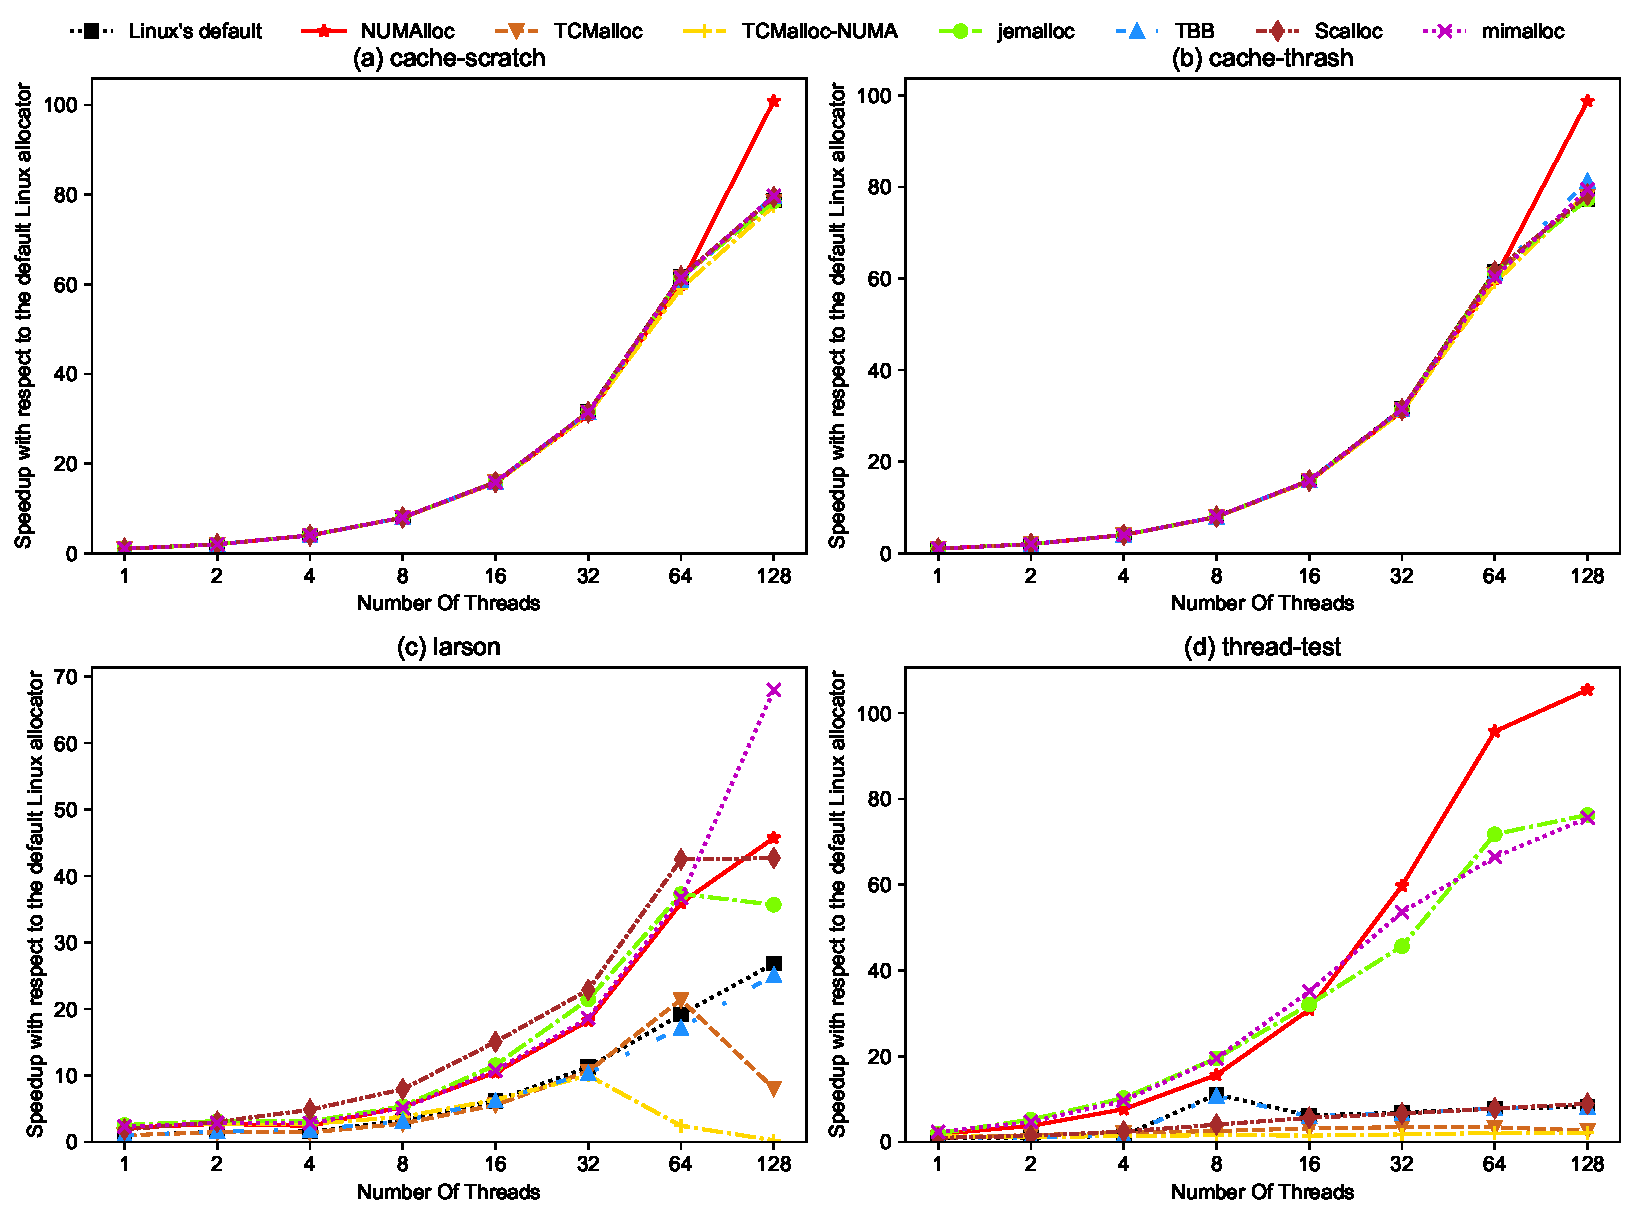
\includegraphics[width=6.1in]{figure/sythentic-scalobility-new.pdf}
    \caption{Scalability evaluation of different allocators.\\ All data is normalized to the runtime of the default Linux allocator with one thread.}
    \label{sythentic-scalability}
\end{figure*}

\begin{figure}[!h]
\centering
\subfloat[Normalized runtime without thread binding for Glibc and TCMalloc, where the lower is the better.]{
  \includegraphics[width=3.2in]{SC2022/figure/threadbinding1.jpg}
}

\subfloat[Normalized runtime with node-interleaved and node-saturate binding for \NM{}, where the lower is the better.]{
  \includegraphics[width=3.2in]{SC2022/figure/threadbinding2.jpg}
}
\caption{Performance impact of thread binding.}
\label{binding-pthread-scalibity}
\end{figure}

\begin{figure}[!ht]
    \centering
    \includegraphics[width=3.2in]{SC2022/figure/hugepage.jpg}
    \caption{Normalized runtime with and without THP for \NM{}.  \label{fig:hugepage}}
\end{figure}

\begin{figure}[!ht]
    \centering
    \includegraphics[width=3.2in]{SC2022/figure/interleavedheap.jpg}
    \caption{Normalized runtime with and without the interleaved heap for \NM{}.  \label{fig:interleavedheap}}
\end{figure}


\subsection{Scalability}
\label{sec:scale}

%We also evaluated the scalability of different allocators. 

To validate the scalability of \NM{}, we use four synthetic applications from Hoard~\cite{Hoard}, including \texttt{threadtest}, \texttt{larson}~\cite{Larson}, \texttt{cache-scratch} and \texttt{cache-slash}, which is also employed by existing work~\cite{Scalloc}. We do not use the same applications in Section~\ref{sec:evaluation}, as they are not scalable by design.
%We have verified blacksholes, bodytrack, canneal, and raytrace.
For instance, raytrace has no performance difference when running with 16 threads or 40 threads.
%Therefore, we are using four synthetic applications from Hoard~\cite{Hoard}, including \texttt{threadtest}, \texttt{larson}~\cite{Larson}, \texttt{cache-scratch} and \texttt{cache-slash}, which is also employed by existing work~\cite{Scalloc}. \texttt{larson} simulates a multithreaded server that could respond to requests from different clients, and \texttt{threadtest} is an application that performs a large number of allocations and deallocations within a specified number of threads. Both \texttt{cache-scratch} and \texttt{cache-thrash} test false sharing issues that can be introduced by allocators, where multiple threads are getting and accessing different objects in the same cache line.  
%Passive false sharing is introduced upon deallocations, where a freed object can be utilized by another thread. In contrast, active false sharing is introduced during the initial allocations, where multiple continuous objects sharing the same cache line are allocated to different threads. The synthetic applications have a better scalability by design than other evaluated applications in the last section. 
%Since other allocators cannot specify the configuration, we only evaluate the scalability with different number of threads. 
In the evaluation, we maximize the number of threads on each node for \NM{}. For instance, 32 threads will use 2 nodes, as each node has 16 cores. For other allocators, we only specify the number of threads, and it is up to the OS to determine the scheduling. 
%The corresponding data is shown in Fig.\ref{sythentic-scalability}. All data are normalized to the data of one thread of the Linux's default allocator, where the higher is better.
 
Fig.\ref{sythentic-scalability} illustrates different allocators' performance speedup with the increasing number of threads. All data is normalized to the runtime of Linux's default allocator under one thread. Overall, \NM{} has the best performance when the number of threads is 128. Its average speedup is $88\times$, compared to Linux's allocator with one thread, while the second-best allocator -- \texttt{mimalloc} -- has $75\times$ speedup. In contrast, the default Linux allocator only has the speedup of $49\times$. That is, \NM{} has the best scalability compared to other allocators.
%When computing the speedup using the data of one thread of each allocator, \NM{}'s average speedup is $65\times$, while the second-best one is $54\times$. 

\NEW{Among these applications, both \texttt{cache-scratch} and \texttt{cache-thrash} test false sharing issues that can be introduced by allocators, where multiple threads access different objects in the same cache line. For both applications, \NM{} has similar scalability compared to other allocators up to 64 threads. But when it comes to 128 threads, \NM{} outperforms all other allocators. According to our investigation, other allocators suffer from false sharing issues while \NM{} avoids the problem and thus has better performance.}
% has a much lower cache miss rate compared to other allocators.}
In these four applications, \NM{} only performs worse than mimalloc for \texttt{larson} with 128 threads. \NEW{\texttt{larson} simulates a multithreaded server that can respond to requests from different clients. In this application, each thread is given a set of objects, and they perform random deallocations and allocations on these objects within a round, and finally pass the objects to the next thread before terminating. Unlike other applications, \texttt{larson} runs for a fixed time and we use a throughput metric (the number of memory allocations per second) to measure the performance. Remote deallocations are quite common for this application, as local objects can be passed to other remote threads. Therefore, the performance of \texttt{larson} is sensitive to the memory recycling mechanisms of the allocator, as observed in the existing work~\cite{Scalloc, scalableallocator}. As discussed in Section~\ref{sec:origin}, remote object's deallocation is managed by the original node's freelist to ensure the locality. This freelist is shared among all threads running on this node, which can become a bottleneck when serving multiple deallocations at the same time. Nevertheless, \NM{} still performs better than most allocators on \texttt{larson} and can scale to 128 threads.}
% Although most deallocations are performed by the allocating thread which occurs on the local node, remote deallocations are also common, as local objects can be passed to other remote threads. Therefore, } 
% we do not know the exact reason for this, but \NM{} is still good enough against other allocators. \NEW{reason!}
% but it performs better against mimalloc for other applications. 
All of these data indicate that \NM{} is scalable to 128 cores. 
%We don't know the exact reason for this.

% \todo{the scalability disadvantage of NUMAlloc at 32 or 64 threads, or > 128 threads}

% \todo{Previous we have analysis of TCMalloc on two cache applications, but I think it's not representative as larson and thread-test}

%Among these applications, \texttt{cache-scratch} tests passive false sharing, and \texttt{cache-thrash} tests active false sharing. False sharing occurs when multiple threads are concurrently accessing different words in the same cache line. 
%Passive false sharing is introduced upon deallocations, where a freed object can be utilized by another thread. In contrast, active false sharing is introduced during the initial allocations, where multiple continuous objects sharing the same cache line are allocated to different threads. 
%For these false sharing tests, we use 100,000 inner-loop, and 100,000 iterations with 8-byte objects.

\begin{comment}
Among these applications, \texttt{cache-scratch} tests passive false sharing, and \texttt{cache-thrash} tests active false sharing. TCMalloc has serious issues of both active and passive false sharing issues, which is the major reason that it does not perform well on both applications. 
\NM{} will not introduce active false sharing, since each thread will get a page of objects initially. Although \NM{} might introduce passive false sharing due to its per-thread cache design, it avoids remote allocations across the node. 
%We believe that is the major reason for its better performance. Other allocators do not have such mechanisms. That is the reason why 
\NM{} is one of the best allocators for \texttt{cache-scratch}, and achieves much better speedup than all other allocators in \texttt{cache-thrash} (30\% faster than the second-best one), as shown in Figure~\ref{sythentic-scalability}. 
\end{comment} 
 %\texttt{larson} is to simulate a multithreaded server that could respond to requests from different clients. \NM{} is around 16\% faster than the second-best allocator--TCMalloc.   \texttt{threadtest} is an application that performs a large number of allocations and deallocations within a specified number of threads. \NM{} is $2.6\times$ faster than the second-best one (jemalloc), when there are 128 threads.
 %Each thread will receive a random number of objects in the beginning, perform a random number of allocation and deallocations to simulate the handler for processing requests, and then pass objects to the next thread. We test \texttt{larson} for 10 seconds with 1,000 objects for 10,000 iterations, where each allocation is between 7 bytes and 2048 bytes. 
 %As shown in Fig.~\ref{sythentic-scalability},  



%Also, it allows to specify how much work to be done between each allocation and deallocation. For \texttt{threadtest}, we use 100 iterations, 1,280,000 allocations, 0 work, and 64-byte objects (for the allocation).  This benchmark will stressfully test the performance overhead of allocation and deallocation. For this application, 
 %since every thread will has its own heap and it only imposes some when getting objects from the shared bag. But \NM{} obtains a number of objects at a time, at the page level, which significant reduce the possibility of contention. 


%On average,  \NM{} is running 79\% faster than the second-best one (Scalloc), and $2.2\times$ faster than the default Linux allocator. Multiple reasons contribute to the good performance of \NM{}: \NM{} imposes very minimal system call overhead, and little synchronization overhead. Also, it introduces less remote accesses than all other allocators, due to its NUMA-aware design. Other allocators have more or less false sharing issue, or incurs remote accesses.  
%\todo{Surprisingly, TCMalloc and  }.



%That is the reason why it has a good performance as the Linux allocator for \texttt{cache-thrash}.

 
\begin{comment}

\begin{figure}[!ht]
    \centering
    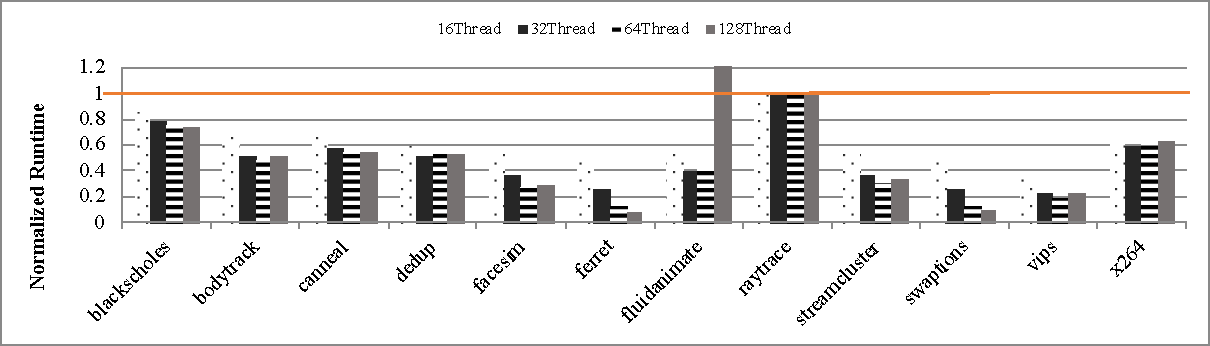
\includegraphics[width=5.5in]{figure/scalobility-pthread.pdf}
    \caption{Normalized performance of Linux's default allocator without binding for PARSEC benchmarks in Machine B}
    \label{pthread-scalibity}
\end{figure}

We will evaluate the scalability on 8threads, 16threads, 32 threads, 64 threads and 128 threads. 
(one node, two node, four nodes, and 8 nodes). 
	
\end{comment}


\subsection{Design Choices}
\label{sec:design}

This section further confirms \NM{}'s multiple design choices.
% all results shown in this section are normalized to the data of the default Linux allocator.  

%Based on our analysis, there are two reasons for this performance speedup. First, a thread will not be migrated to a different core, avoiding unnecessary remote accesses caused by cross-node migration, as further discussed in Section~\ref{sec:intro}. Second, \NM{}'s thread binding balances the workload, thus reducing the congestion of interconnect or one memory controller.
\subsubsection{Choices of Thread Binding}
\label{sec: threadbinding}

% \begin{figure*}[!h]
%     \centering
%     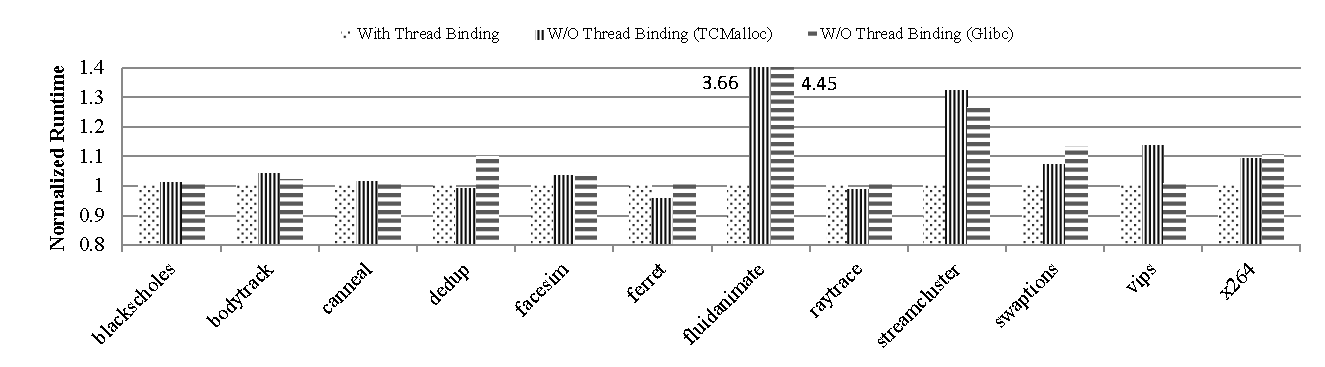
\includegraphics[width=6in]{figure/WO-pthread-binding3.pdf}
%     \caption{Normalized runtime with and without node-balanced thread binding for Glibc and TCMalloc.} 
%     \label{binding-pthread-scalibity}
% \end{figure*}

% \begin{figure*}[!ht]
%     \centering
%     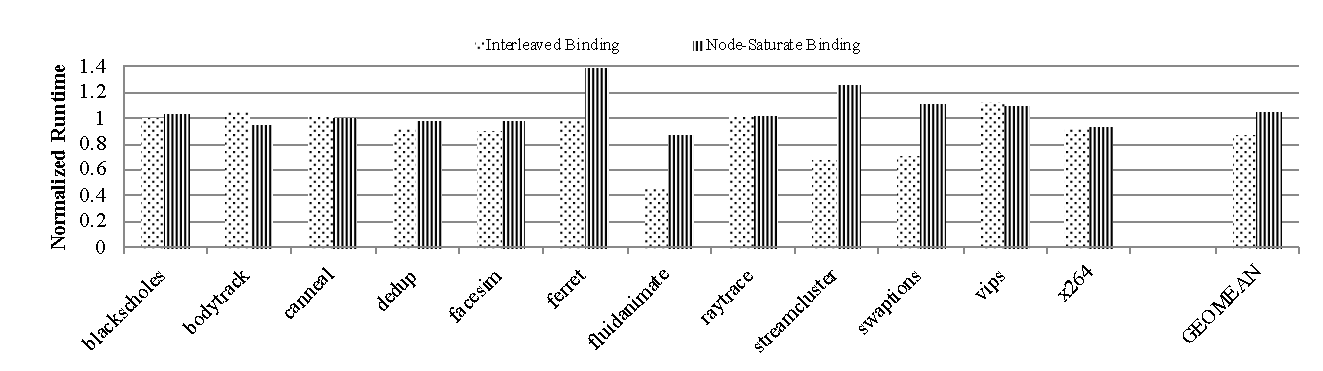
\includegraphics[width=5.5in]{figure/binding-policy.pdf}
%     \caption{ Node-Interleaved vs. Node-Saturate binding for Glibc, where results are normalized to those without binding.}
%     \label{fig:binding-policy}  
% \end{figure*}

\NEW{\NM{}'s memory management is based on binding, including thread binding and memory binding. We believe such bindings benefit the performance and open up other design opportunities, such as origin-aware memory management, metadata allocation and incremental sharing. The combination of all design choices makes \NM{} a faster and more efficient allocator. Therefore, we cannot evaluate the impact of thread binding by directly disabling it on \NM{} since other designs depend on it. To overcome this problem, we implement a thread binding library that allows other allocators to enable binding.}
Fig.\ref{binding-pthread-scalibity}(a) shows the \NEW{impact of thread binding on} two allocators, Glibc and TCMalloc.
% Fig.\ref{binding-pthread-scalibity}(a) shows the performance difference without thread binding for two allocators, Glibc and TCMalloc.
The results are normalized to the data with thread binding of each allocator, respectively, \NEW{so we omit the ones with thread binding. Thus, this figure can be considered to show how much slower it would run without thread binding.}
% We cannot evaluate \NM{} directly, since its mechanisms are tightened to thread binding, such as incremental sharing, origin-aware memory management and metadata allocation. 
Here we use the node-interleaved binding. As shown in Fig.\ref{binding-pthread-scalibity}(a), the thread binding improves the performance significantly for some applications. For instance, \texttt{fluidanimate} runs around $4.45\times$ faster on Glibc and $3.66\times$ faster on TCMalloc with the node-balanced thread binding. Similarly, \texttt{streamcluster} runs around 20\% and 30\% faster than the corresponding one without the binding. 
\NEW{We further use \texttt{perf}~\cite{perfweb} to analyze the reasons for the significant performance improvement of these two applications. The results confirm that remote accesses are significantly reduced with thread binding, mainly due to the elimination of thread migration. Interestingly, the cache miss rate also decreases with thread binding. Overall, thread binding will benefit the performance of most applications without hurting others,} 
% This clearly indicates that the thread binding will benefit the performance overall
which should be included in the memory allocator by default. 

% In particular, threads are bound to different nodes in a round-bin way, called node-balanced binding, which is the same as \NM{}.

We also compare two types of thread binding: node-interleaved or node-saturate thread binding. In node-saturate binding, we bind the maximum possible number of threads (same as the number of cores) to a node and then switch to the next node. As shown in Fig.\ref{binding-pthread-scalibity}(b), the node-interleaved thread binding is almost always better than node-saturate thread binding, except for \texttt{bodytrack}. On average, node-interleaved binding is around 19\% faster than node-saturate one for these evaluated applications. This indicates that people should use node-interleaved binding, if they would like to employ all hardware cores. However, if they only want to use partial cores, then the node-saturate binding could be a better choice. \NM{} allows users to adjust the binding option based on their needs.

% , proving the effectiveness of Node-Balanced thread binding.

\subsubsection{Impact of Transparent Huge Pages}

As discussed in \ref{sec:hugepages}, it's beneficial to embrace the transparent huge page support in modern systems. We evaluate the performance impact of transparent huge pages. The results are shown in Fig.~\ref{fig:hugepage}. When integrating with transparent huge pages, \NM{} achieves significantly better performance for \texttt{vips}, where it is running 16\% faster. On average, transparent huge pages improve the performance by about 2.62\%. There are no applications that run slower with huge pages. This clearly indicates that it is beneficial to enable transparent huge pages for the NUMA architecture, especially when \NM{} is used. 
Although \NM{} may increase its memory overhead from 2\% to 10\% when using huge pages, as shown in Table~\ref{tab:memory_consumption}, the memory overhead is still acceptable, given the hardware trend of increasing memory capacity.  


\subsubsection{Impact of Interleaved Heap} 
\label{sec:interleavedheap}

We also evaluate the potential benefit of the interleaved heap. The performance data is shown in Fig.\ref{fig:interleavedheap}. 
% Note that we have evaluated all PARSEC applications listed in Section~\ref{sec:performance}.
Based on the figure, we have the following conclusion: the interleaved heap will benefit (or at least has no harmful impact on) the performance for most applications. In particular, it improves the performance significantly on \texttt{fluidanimate} and \texttt{streamcluster}.  However, applications having a large portion of time spent in the serial phase, such as \texttt{canneal} and \texttt{raytrace}, may hurt the performance with the interleaved heap support. These two applications share the same property that they have a larger portion of the first serial phase. With the interleaved heap, \NM{} allocates the memory from different nodes interleavedly for the serial phase, instead of from the local node (based on the default first-touch policy). That is, some private objects allocated in a remote node may introduce unnecessary performance overhead due to remote accesses. Currently, we do not know why swaptions has a large \NEW{negative} performance impact when the interleaved heap is employed, whose performance can change dramatically when adding one \NEW{meaningless code line (declaration and assignment of a \texttt{volatile} variable) or changing the compilation flags}. We will keep investigating this. 
%Further, upon each allocation, \NM{} checks the callstack to confirm whether an allocation is from a potentially shared heap, which also introduces some overhead. Therefore, the interleaved heap will be enabled by default, unless programmers know that it will not benefit the performance.

Programmers can choose to enable or disable interleaved heap based on the applications. A simple metric is to use the portion of the serial phase inside multithreaded applications. For applications that are mostly running in the serial phase, turning off the interleaved heap support may be a better choice. That is, the interleaved heap will harm the serial execution, but may benefit the parallel execution because of its load balance. It is easy to turn on/off the interleaved heap via a compilation flag or the environment variable.  

\subsubsection{Impact of Origin-aware Deallocation}

\NM{} adopts an origin-aware deallocation that always returns the object to its original thread's or node's heap. We further verified the effect of this design and the results show that \NM{} runs 1.7\% slower if we do not consider the origin of freed objects. The details are omitted due to the space limitation. 

% \todo{other design choices: THP's impact on performance, origin-based deallocation, autonuma's impact...}

%, except applications with a large portion of serial phase (e.g., \texttt{canneal} and \texttt{raytrace})

%The interleaved heap could be utilized to avoid load imbalance issue for shared objets. 

%However, there are two issues for the interleaved heap. First, the allocator may not know whether an object is shared or not at the first time. Therefore, all objects that are allocated in the main heap (before creating any child thread) will be treated as the shared heap. Second, some applications are spending too much time in the serial phase, where the interleaved heap cannot benefit the performance for the serial phase. 





%figure ~\ref{parsec-no-interleaved-perf} we show some performance results of some applications that got significant different values after we shut down interleaved heap for \NM{}. We can see that for some applicatios with less data sharing between threads like ratrace and canneal, \NM{} could got significant improvements due to its low overheads and proper memory management. But for some other applications with intensive memory operations and sharing like fluidanimate, shutting down interleaved heap could hurt performance, since interleaved heap could help to distributed resource contention evenly over multi-nodes and then got low overheads.

%\subsubsection{Selective Huge Pages} 
%\label{sec:hugepage}

%Since the machine utilizes transparent huge pages by default, we evaluate the performance impact of huge page support on another machine with 2 NUMA-node, without enabling the transparent huge pages.
% A, the 2-node machine. We only utilize PARSEC applications for this evaluation. 

%\begin{figure}[!h]
%    \centering
%    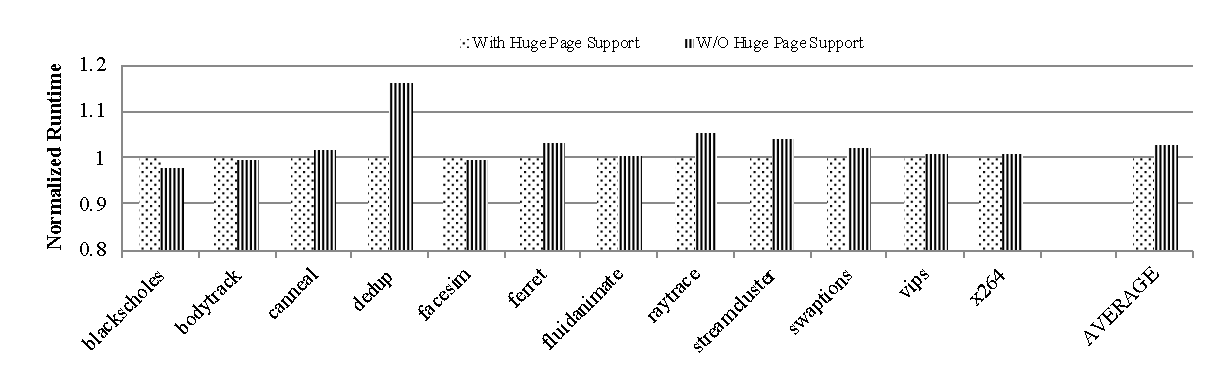
\includegraphics[width=3.2in]{figure/hugepage.pdf}
%    \caption{Normalized runtime with and without selective huge pages.}
%    \label{fig:hugepage}
%\end{figure}

%The results are shown in Figure~\ref{fig:hugepage}. When integrating with selective huge pages, \NM{} achieves a significantly better performance for \texttt{dedup}, where the performance difference is around 15\%. On average, the selective huge pages improves the performance of all evaluated applications about 2.5\%, and will not hurt the performance. This clearly indicates that it is beneficial to have selective huge pages for the NUMA architecture, especially given the fact of increasing memory size of hardware trend.  



\section{Limitation}
\label{sec:limit}

This section describes some limitations of \NM{}. First, \NM{} may consume more memory than some popular allocators, especially when transparent huge pages are enabled. \NM{} currently allocates a big chunk (larger than a huge page) from the OS, then the OS will satisfy the memory allocations with huge pages when transparent huge pages are enabled. Although this method reduces the possible system call overhead and enjoys the performance benefits caused by reducing TLB misses, it does introduce more memory consumption. That is, the whole huge page will be wasted even if applications only use a small portion of huge pages. However, we believe that this shortcoming is tolerable, when memory is not the major concern. 
%As shown in Figure~\ref{fig:remoteAccess}, \NM{} significantly reduces the number of TLB misses by trading with medium memory consumption. 


Second, \NM{}'s interleaved heap cannot always achieve the performance improvement due to the following reason. Although the interleaved heap may avoid memory controller congestion caused by concurrent accesses from multiple child threads, it introduces unnecessary overhead for the initial thread since it is forced to have some remote accesses. 
%(2) Although \NM{} avoids the change of programs to utilize the interleaved heap, it imposes additional overhead to identify the callsites for potentially shared objects. 
Therefore, users should decide whether to enable the interleaved heap or not. However, this is an easy task, since the interleaved heap may have a harmful impact when the serial phase is a big portion of the execution. Therefore, we think that this shortcoming is totally acceptable given its predictability. 

\NM{} is built based on the thread binding, where people may worry about its conflict with the OS scheduler. In fact, based on our understanding, this should not be a big issue due to the following reasons. First, \NM{}'s thread binding does not exclude OS's scheduling, as it only binds a thread to a node. Second, \NM{} allows users to adjust the binding flexibly, although currently \NM{} only supports node-interleaved and node-saturate binding. But adding more flexible binding will be just pure engineering effort. Third, the thread binding is even suitable for server applications with thousands of threads, as \NM{}'s binding balances the workload among different physical nodes. 
%Based on our analysis, the memory consumption is caused by \NM{}'s bag mechanism, especially with transparent huge page support. Currently, \NM{} employs one MB as a bag, which indicates that objects of each size will occupy at least of 1 MB, when transparent huge page support is enabled. Further, \NM{}'s design achieves a fast lookup on the metadata, but will utilize more memory unfortunately. We will investigate whether reducing the size of a bag could help reduce the memory consumption in the future.

%The second limitation is that \NM{} will crash less often by preallocating a huge chunk of memory from the OS in the beginning. If an invalid reference is landed within a pre-allocated range, a program will not crash, different from other allocators. Instead, \NM{} aims to achieve the high performance over the reliability. Therefore, we believe that this limitation is acceptable.  
\begin{comment}
\todo{NUMAalloc may not suitable for the situation for the system has thousands of threads. But maybe still okay, as these threads are balanced distributed to different nodes.

NUMAlloc can be useful for certain applications and system configurations and appears to be well-crafted. 

Maybe we could say that numa support is a daunting task, but it is actually not. This paper shows how to use and embedded these mechanisms in order to choose a better result. 
Interleaving shared objects similarly can make sense (e.g. as in the applications used in the evaluation of the paper) but is not easy to accept that it will universally work well or better than other techniques. As a different case from the one above, consider a server where tens-hundreds of different applications are running, possibly in containers/VMs, starting and finishing dynamically. What does interleaving shared objects say for such cases?

}

\end{comment}

\section{Related Work}

\label{sec:related}

This section discusses some related work with \NM{}. 

\paragraph{General Purpose Allocators}
 There exists a large number of allocators~\cite{dlmalloc,Hoard,tcmalloc,jemalloc,Scalloc}, but they are not designed for the NUMA architecture. Based on the management of small objects, allocators can be further classified into multiple types, such as sequential, BiBOP, and region-based allocators~\cite{Gay:1998:MME:277650.277748,  DieHarder}. Region-based allocators are suitable for special situations where all allocated objects within the same region can be deallocated at once~\cite{Gay:1998:MME:277650.277748}. For sequential allocators, subsequent memory allocations are satisfied in the continuous memory area, such as the Linux allocator~\cite{dlmalloc} and Windows allocator~\cite{DieHarder}. That is, objects of different sizes can be placed continuously. For BiBOP-style allocators, one or multiple continuous pages are treated as a ``bag'', holding objects with the same size class. \NM{} also belongs to BiBOP-style allocators, as do many other high-performance and security-focused allocators ~\cite{tcmalloc, jemalloc, Hoard, Scalloc, DieHarder}. But \NM{}
  proposes multiple special designs for the NUMA architecture.
 
 %\todo{Adding supermalloc and mimalloc}

\paragraph{NUMA-aware Allocators} TCMalloc-NUMA adds additional node-based freelists and free spans to store freed objects and pages belonging to the same node~\cite{tcmallocnew}, which is similar to \NM{}. It also invokes the \texttt{mbind} system call to bind physical memory allocations to the node that the current thread is running on, which is similar to JArena~\cite{yang2019jarena}. But JArena requires the co-design of applications, runtime system and the underlying OS, which is not transparent to users~\cite{yang2019jarena}. Also, both of them do not support the interleaved heap, invokes too many \texttt{mbind} system calls, and does not handle the metadata's locality. nMART proposes a NUMA-aware memory allocation for soft real-time system~\cite{kim2013node}. It proposes a node-oriented allocation policy to minimize the access latency, and ensures temporal and spatial guarantee for real-time systems. nMART requires the change of the underlying OS, which is different from \NM{}. nMART also has a different target as \NM{} that tries to meet the time requirement of real-time systems, and \NM{} focuses more on the performance. mimalloc also supports NUMA memory management~\cite{mimalloc}. It records the associated numa node for each segment, and tries to obtain a segment from the same node when reusing segments between threads. mimalloc proposes a page-based freelist that could only serve a thread at a time~\cite{mimalloc}, where all objects will be returned to the same page-based freelist upon deallocations. By allocating physical memory of each page locally, mimalloc have achieved some level of the locality. However, mimalloc cannot ensure local allocations when a thread is migrated. \NM{} overcomes these issues, and further balance the memory accesses from different nodes via its node-balanced thread binding and interleaved heap. 


\paragraph{NUMA-Aware Java Heap Management} Some approaches that focus on improving the performance of Java applications, but they are not general purpose memory allocators. Ogasawara et al. focus on finding the preferred node location for JAVA objects during the garbage collection and memory allocations~\cite{Ogasawara}, via thread stack, synchronization information, and object reference graph. Tikir et al. propose to employ hardware performance counters to collect the runtime information of Java applications, and then migrate an object to the closet node with most accesses~\cite{1419934}. 
NumaGiC reduces remote accesses in garbage collection phases with a mostly distributed design so that each GC thread will mostly collect memory references locally, and utilize a work-stealing mode only when no local references are available~\cite{NumaGiC}.


\paragraph{Combination of Task Scheduling and Memory Management} Redline integrates task scheduling and memory management inside the OS level~\cite{Redline}, to support interactive applications. 
Majo et al. propose to consider both data locality and cache contention to achieve better performance for the NUMA applications~\cite{Majo:2011:MMN:1993478.1993481}. Wagle observed that dynamic memory allocations, thread placement and scheduling, memory placement policies, OS configurations may help improve the query performance of in-memory databases~\cite{wagle2015numa}.  Majo et al. propose to set task-to-thread affinity, and pin threads to specific cores to achieve a better performance~\cite{Majo:2015:LPC:2688500.2688509}. Diener proposes a new kernel framework to combine task management and memory management together to achieve better performance~\cite{diener2015automatic}. 
Debes et al. propose the combination of enhanced work-pushing and deferred allocation together to improve the performance for data-parallel tasks, but focusing on special programming models~\cite{DBLP:conf/IEEEpact/DrebesPH0D16}. They inspire \NM{}'s binding-based memory management. But \NM{} is the first work that combines both together inside a memory allocator. 

\paragraph{Huge Page Support of Memory Allocators}
SuperMalloc~\cite{supermalloc} is possibly the first allocator that supports huge pages. To reduce memory wastes, it only utilizes huge pages for large objects. LLAMA~\cite{LLAMA} allocates memory objects with the similar expire time to the same huge page, and utilizes machine learning to identify the life-time of memory objects from each callsite. That is, LLAMA requires the profiling to adjust its memory allocations for each application, which could be expensive or inconvenient to do so.  TEMERAIRE~\cite{TEMERAIRE}, which is the default setting of TCMalloc, maximizes the usage of huge pages. It allocates big objects from huge pages, and also allocates small objects from partially-filled huge pages. \todo{That is, small allocations before a medium/large allocation (e.g., larger than 1MB) will be satisfied from small pages. }    

Instead, \NM{} allocates all memory (except the interleaved heap) from huge pages,  but reducing the fragmentation by making different size classes to share the same huge page. Overall, \NM{}'s mechanism is simpler but easy to implement, which could combine with LLAMA and TEMERAIRE together. In theory, \NM{} may introduce higher overhead, as it utilize huge pages for all memory objects, preventing the returning of huge pages back to the OS. 



\paragraph{NUMA Libraries}
Cantalupo et al. propose multiple APIs that allow users to manage their memory in fine granularity by combining with multiple existing system calls~\cite{cantalupo2015memkind}. However, they are not targeting a general purpose allocator, since it requires programmers to manage the memory explicitly.  Majo et al. propose multiple source-code based  algorithmic changes in order to improve data sharing and memory access patterns for NUMA architectures~\cite{6704666}. Williams et al. propose to group data structures that can be migrated together with arenas~\cite{WilliamsI0L18}. 
Shoal also proposes a set of APIs that allow the user to specify memory access patterns~\cite{Kaestle:2015:SSA:2813767.2813787}. 
%Then it could automatically replicate or distribute the memory to different NUMA nodes automatically. 
But both of them need significant manual effort to employ this. 
%XPV extends virtualization technique by considering NUMA-topology and extending virtualization to SRLs ~\cite{Bui:2019:EPV:3302424.3303960}.

%\todo{Changing the following two paragraphs}
\paragraph{Reactive Systems for NUMA Architecture} Some systems migrate tasks or physical pages reactively based on memory access patterns or other hardware characteristics~\cite{simplenuma, Blagodurov:2011:CNC:2002181.2002182, AutoNUMA, Dashti:2013:TMH:2451116.2451157, Lepers:2015:TMP:2813767.2813788}. 
%They improve the performance automatically without human involvement. However, these systems impose additional overhead (sometimes unnecessarily)  by migrating tasks or physical pages reactively. Further, a reactive approach cannot reduce remote accesses by the migration, if objects of the same page are concurrently accessed by multiple threads in multiple nodes~\cite{Gaud:2014:LPM:2643634.2643659}. 
\NM{} belongs to a proactive approach that does not require explicit and page migration, which is complementary to these reactive systems. 
%It is possible to combine these two together to achieve better performance. 

%The second approach relies on programmers to manage memory allocations and task assignments explicitly~\cite{Kaestle:2015:SSA:2813767.2813787, Lin:2016:MTP:2872362.2872401, Majo:2017:LPC:3057718.3040222}. Although they could improve the performance greatly, they typically require significant human effort to rewrite the programs, where legacy systems cannot benefit automatically. 

\section{Conclusion}
\label{sec:conclusion}

\NM{} is a memory allocator that is specially designed for the NUMA architecture. Applications can be linked to \NM{} directly, without the change of code and the recompilation. \NM{} is different from existing memory allocators, as it is the first binding-based allocator. 
On top of it, it further proposes origin-aware memory management and incremental sharing to improve the locality and exploit huge pages. 
% It further proposes threads-shared incremental allocation and origin-aware memory management to improve the locality. 
Based on our extensive evaluation, \NM{} achieves a significantly better performance than other popular allocators on the NUMA architecture, which is running \NEW{15.7\%} faster (and up to $6.8\times$ faster) than the second-best allocator.
%\NM{} is available at https://github.com/XXX. 

% \todo{the number order of reference has a issue, check 49, 50 later}

\bibliographystyle{IEEEtranS}
\bibliography{ref,emery,tongping}

\end{document}
